\documentclass{bachelor_thesis}
\usepackage{polski}
\usepackage{blindtext}
\usepackage{graphicx}
\usepackage{caption}
\usepackage{subcaption}
\usepackage{natbib}
\usepackage[utf8]{inputenc}

\author{Kamil Kolasa}

\nralbumu{405765}

\title{Badanie własności różniczkowo rotujących gwiazd zwartych}

\tytulang{Properties of differentially rotating compact stars}

\kierunek{astronomia}

\opiekun{dr hab. Doroty Rosińskiej\\Katedra Astrofizyki Teoretycznej\\Obserwatorium Astronomiczne UW}

%\dziedzina{13.200}
%\dziedzina{13.7 Astronomia}

\date{lipiec 2021}

\keywords{gwiazdy neutronowe - gwiazdy dziwne - sztywna rotacja - różniczkowa rotacja - stabilność}



\begin{document}


    \maketitle
    \let\cleardoublepage\clearpage
    
    \begin{abstract}
\hspace{.45cm} Gwiazdy zwarte są ostatnimi etapami ewolucji gwiazd. Ich gęstości są wielokrotnie większe niż w termojądrowo aktywnych gwiazdach. Należą do nich m.in. gwiazdy neutronowe i hipotetyczne gwiazdy kwarkowe, które dzięki wyjątkowo szybkiej rotacji mogą osiągać większe masy niż nierotujące gwiazdy o tym samym równaniu stanu. Różniczkowa rotacja pozwala na osiąganie dużo większych mas maksymalnych niż rotacja sztywna. Wciąż jednak nierozstrzygnięte pozostaje zagadnienie stabilności masywnych różniczkowo rotujących gwiazd zwartych względem zapadania do czarnej dziury w dynamicznej skali czasowej. Takie gwiazdy powstałe w wyniku koalescencji dwóch gwiazd neutronowych lub z zapadającego się jądra masywnej gwiazdy podczas wybuchu supernowej mogą być silnym źródłem fal grawitacyjnych.\\
\indent Celem mojej pracy było zbadanie własności różniczkowo rotujących gwiazd zwartych dla szerokiego zakresu mas, momentów pędu i gęstości oraz kilku wybranych stopni różniczkowej rotacji. Stosując relatywistyczny kod FlatStar przeprowadziłem masowe obliczenia stacjonarnych modeli różniczkowo rotujących gwiazd neutronowych i kwarkowych wyznaczając m.in. ich masy maksymalne w zależności od stopnia różniczkowej rotacji. Przeprowadziłem wstępną analizę stabilności masywnych gwiazd zwartych stosując kryterium analogiczne do kryterium używanego dla sztywno rotujących gwiazd neutronowych i kwarkowych. Do tej pory nie została przeprowadzona tego typu analiza dla bardzo masywnych gwiazd o kształtach toroidalnych. Pokazałem, że najmasywniejsze konfiguracje mogą być stabilizowane dzięki różniczkowej rotacji. Wyznaczone ciągi marginalnie stabilnych konfiguracji będą punktem wyjścia do przeprowadzenia hydrodynamicznej analizy stabilności. Dla tych konfiguracji sprawdziłem istnienie pewnych uniwersalnych zależności między masą a momentem pędu pokazując, że te same zależności są spełnione dla szerszych niż jak dotąd rozpatrywane zakresów, mają jednak inny przebieg dla gwiazd kwarkowych.

     \end{abstract}

\newpage
\thispagestyle{empty}
\newpage
 \thispagestyle{empty}
 \begin{minipage}{10cm} \hfill
 \end{minipage}%
 \begin{minipage}{5cm}
  \vspace{18.5cm}
  { \textit{Serdeczne podziękowania dla dr hab. Doroty Rosińskiej, za pomoc i cierpliwość w trakcie przygotowywania tej pracy.
}}
\end{minipage}
    
   \tableofcontents
    
    \chapter{Wstęp}
        \section{Gwiazdy neutronowe - podstawowe informacje}
        W roku 1932 James Chadwick odkrył neutron. Już dwa lata później Walter Baade i Fritz Zwicky zapostulowali istnienie gwiazd powstających w wybuchach supernowych, w których grawitacyjne zapadanie mogłoby zostać powstrzymane jedynie przez ciśnienie zdegenerowanych neutronów. Te obiekty zostały nazwane gwiazdami neutronowymi. Niedługo później wyznaczono ich masę i promień, poprzez obliczenia oparte o Ogólną Teorię Względności. Realistyczne równania budowy zwartych obiektów nazwano równaniami Tolmana-Oppenheimera-Volkoffa (\citealp{Tolman1934}, \citealp{Volkoff1939}, \citealp{Tolman1939}), w skrócie TOV.\\
        \indent Jednak ówcześnie sygnał pochodzący od gwiazd neutronowych uznawany był za zbyt słaby do zaobserwowania, a obiekty te pozostawały hipotetycznymi aż do roku 1967, w którym Antony Hewish i jego doktorantka Jocelyn Bell zaobserwowali w Mgławicy Kraba regularne pulsy radiowe trwające $0,04$ s w odstępach $1,3373$ s. Okazało się, że były one emitowane przez pulsar PSR 1919+21. Pulsary są wyjątkowymi przypadkami gwiazd neutronowych, o szybkim tempie rotacji i polach magnetycznych na tyle silnych, że emitują wiązki promieniowania elektromagnetycznego ze swoich biegunów. Za to odkrycie Hewish został nagrodzony Nagrodą Noble'a w dziedzinie fizyki. W 1974 roku Joseph Taylor oraz Russell Hulse odkryli pierwszy podwójny układ pulsarów -- PSR B1913+16. To odkrycie również zostało nagrodzone Nagrodą Noble'a, w 1993 roku. Według Ogólnej Teorii Względności taki układ powinien emitować fale grawitacyjne oraz stopniowo zacieśniać orbitę. Owe zacieśnianie rzeczywiście zostało zaobserwowane i dokładnie zgadzało się z przewidywaniami OTW. Był to kolejny dowód na słuszność teorii Einsteina, a także pierwszy pośredni dowód na istnienie fal grawitacyjnych, których bezpośrednie obserwacje nastąpiły dopiero 40 lat później. Pierwsza detekcja nastąpiła w 2015 roku, z kolei w sierpniu 2017 roku detektory LIGO i VIRGO zarejestrowały sygnał w postaci fal grawitacyjnych GW170817, pochodzący od dwóch zderzających się gwiazd neutronowych.\\
        \indent Gwiazdy neutronowe powstają w wyniku wybuchu supernowej. Jest to ostatni etap ewolucji gwiazd ciągu głównego o masach $8-10\textrm{ M}_\odot$. W trakcie zachodzenia syntezy do coraz wyższych pierwiastków wewnątrz gwiazdy, jej jądro zaczyna ostatecznie składać się z żelaza. Ponieważ dalsze reakcje termojądrowe są niekorzystne energetycznie, obiekt traci swoje paliwo i zaczyna zapadać się grawitacyjnie. Po przekroczeniu gęstości jądra atomowego $4\cdot 10^{17}$ kg/m$^3$ zapadanie zostaje zatrzymane przez ciśnienie zdegenerowanych neutronów, podczas gdy zewnętrzne warstwy gwiazdy zostają odrzucone. Obserwowany jest wybuch supernowej. Pozostałość po wybuchu jest właśnie gwiazdą neutronową o masie ok. $1-3\textrm{ M}_\odot$, promieniu ok. $10-30\textrm{ km}$ oraz gęstości przewyższającej $4\cdot 10^{17}$ kg/m$^3$. Spośród wszystkich gwiazd neutronowych wyróżnia się wspomniane wyżej pulsary, a także magnetary -- posiadają one jeszcze silniejsze pola magnetyczne rzędu ponad $10^{10}$ T. Wyodrębniane są także pulsary milisekundowe, o wyjątkowo krótkich okresach obrotu z zakresu $1-10$ ms.\\
        \indent  Obecnie znanych jest ponad 2500 gwiazd neutronowych, z czego większość z nich to pulsary, obserwowane głównie w częstościach radiowych i rentgenowskich. Najszybciej rotującym znanym pulsarem jest PSR J1748-2446ad, rotujący z częstotliwością $716$ Hz i okresie obrotu $1,386$ ms. Z kolei najmasywniejszą poznaną gwiazdą neutronową jest pulsar PSR J0740+6620 o masie ok. $2,17$ $M_\odot$, będący w układzie podwójnym z białym karłem. Układ jest możliwy do zaobserwowania jako sygnał elektromagnetyczny.
        \section{Gwiazdy dziwne - podstawowe informacje}
        Ponieważ gęstości centralne gwiazd neutronowych przewyższają gęstość jądrową, warunki panujące wewnątrz nich są obecnie niemożliwe do odtworzenia w laboratorium. Nie istnieje zatem żadne zweryfikowane doświadczalnie równanie stanu gwiazd neutronowych, jednak jest wiele proponowanych. Jednym z nich jest hipoteza gwiazd kwarkowych (dziwnych). W 1971 r. zapostulowano przez \cite{Bodmer1971}, że materia dziwna zbudowana z kwarków \textit{up}, \textit{down} i \textit{strange} może być podstawowym stanem materii przy zerowym ciśnieniu i zerowej temperaturze. Z kolei istnienie gwiazd dziwnych zostało zaproponowane przez \cite{Witten1984}. Według niego wewnątrz gwiazd neutronowych mogłyby zajść warunki korzystne dla przejścia fazowego do materii kwarkowej, z której w większości miałaby składać się gwiazda. Jednak z powodu wspomnianych ograniczeń nie wiadomo, czy ta hipoteza jest słuszna. Należy jednak zauważyć, że w ramach równania stanu gwiazd dziwnych mogą istnieć m.in. gwiazdy o promieniach mniejszych niż te możliwe do osiągnięcia dla któregokolwiek z równań stanu gwiazd neutronowych. Gdyby zatem udało się zaobserwować obiekt o tak małym promieniu i masie gwiazdy neutronowej, mógłby on zostać uznany za gwiazdę dziwną. Jak dotąd taki obiekt nie został zaobserwowany.
        \section{Motywacja i cel pracy}
        Celem poniższej pracy było zbadanie właściwości różniczkowo rotujących gwiazd neutronowych, wyznaczenie możliwych do osiągnięcia maksymalnych mas i oszacowanie przedziałów stabilności względem zapadania do czarnej dziury w dynamicznej skali czasowej. Chociaż jak dotąd nie znaleziono dokładnego kryterium stabilności dla gwiazd zwartych rotujących różniczkowo, istnieją badania (\citealp{Weih2018}, \citealp{Bozzola2018}) wskazujące na to, że kryterium dla gwiazd rotujących w sposób sztywny (\citealp{Friedman1988}) może być dobrym jego przybliżeniem dla małych stopni różniczkowej rotacji i momentów pędu. Ponadto, sprawdzone zostały pewne uniwersalne dla badanych obiektów prawa zapostulowane przez \cite{Bozzola2018}.\\
        \indent Koalescencja dwóch gwiazd neutronowych lub zapadanie jądra masywnej gwiazdy może prowadzić do utworzenia różniczkowo rotującej gwiazdy neutronowej bądź kwarkowej. Badania stacjonarnych modeli takich obiektów pokazują, że mogą one osiągać nawet czterokrotnie większe masy niż masa maksymalna gwiazd nierotujących. (\citealp{Rosinska2017}). Wraz z usztywnieniem rotacji gwiazda może zapaść się do czarnej dziury. Taki scenariusz może być interesującym źródłem fal grawitacyjnych (\citealp{Giacomazzo2011}). Jednak wciąż pozostaje otwartym pytanie, czy najmasywniejsze przewidywane gwiazdy zwarte mogą być tymczasowo stabilizowane przez różniczkową rotację. Ponadto sygnały odbierane przez obecnie działające, a także przyszłe detektory fal grawitacyjnych mogą być produkowane nie tylko przez gwiazdy neutronowe i kwarkowe. Znajomość badanych w tej pracy obszarów stabilności oraz pozostałych parametrów może w przyszłości pomóc lepiej ustalić, czy odbierany sygnał pochodzi od gwiazdy neutronowej, gwiazdy kwarkowej czy od czarnej dziury.\\
        \indent Układ tej pracy jest następujący: w rozdziale 2. omówione zostaną najważniejsze własności gwiazd zwartych rotujących sztywno i różniczkowo. W podrozdziale 2.1. omówię użyte przeze mnie w obliczeniach równania stanu materii w gwiazdach neutronowych i dziwnych, w podrozdziale 2.2. omówię gwiazdy nierotujące, w podrozdziale 2.3. rotujące sztywno i różniczkowo. Podrozdziały 2.4.-2.6. dotyczą mas maksymalnych rotujących gwiazd zwartych, przedziałów ich stabilności oraz pewnych uniwersalnych zależności dla marginalnie stabilnych konfiguracji. Rozdział 3. zawiera opis użytego do obliczeń relatywistycznego kodu FlatStar, najważniejsze parametry oraz metodologię badań. W rozdziale 4. zaprezentowane i omówione zostały wyniki przeprowadzonych przeze mnie obliczeń dla gwiazd neutronowych i kwarkowych rotujących sztywno oraz rózniczkowo. Rozdział 5. jest podsumowaniem pracy.
    \chapter{Gwiazdy zwarte -- własności, rotacja i stabilność}
        \section{Równania stanu}
        We wnętrzach gwiazd neutronowych panują gęstości większe niż $4\cdot 10^{14}$ g/cm$^3$, a energia termiczna $E_T$ jest dużo mniejsza od energii Fermiego $E_F$. W takim przypadku można przyjąć, że temperatura panująca w gwieździe $T=0$ K. Zdegenerowaną materię neutronową można opisać barotropowym równaniem stanu:
        \begin{equation}
            P=P(\rho)
            \label{EqBar},
        \end{equation}
        gdzie $P$ jest ciśnieniem, a $\rho$ gęstością wewnątrz gwiazdy. \\
        \indent W wielu pracach dotyczących gwiazd neutronowych (m.in. \citealp{Cook1992}, \citealp{Cook1994a}, \citealp{Baumgarte2000}, \citealp{Giacomazzo2011}, \citealp{Rosinska2017}) jako równania stanu używa się równania politropy:
        \begin{equation}
            P(\rho)=K\rho^{\Gamma},
            \label{EqPol}
        \end{equation}
        gdzie K jest stałą politropy, a $\Gamma$ to wykładnik politropy. W tej pracy zbadane zostały parametry gwiazd neutronowych opisanych równaniem politropy o wykładniku $\Gamma=2$, stała politropy została przyjęta jako $K=1$.\\
        \indent Gęstości we wnętrzach gwiazd neutronowych są większe od gęstości jądra atomowego. Obecnie nie jest znany stan podstawowy materii w gęstościach przekraczających gęstość jądrową. Istnieje wiele hipotez próbujących opisać wnętrza gwiazd neutronowych, co pokazuje schematyczny Rysunek \ref{RysEOS_examples}. Mogą istnieć w nich np. warstwy nadciekłe bądź nadprzewodzące, a niektóre modele przewidują kondensację pionów bądź kaonów w centrum. Innym niż politropowe równanie stanu jest równanie stanu gwiazd składających się z materii kwarkowej (dziwnej). Według tej hipotezy, rozważane gwiazdy składają się w większości z kwarków u, d oraz s otoczonych cienką skorupą. Taka konfiguracja nazywana jest modelem worka (ang. \textit{MIT Bag model}), ponieważ według \cite{Haensel2007} kwarki są samozwiązane. Gdyby znalazły się poza workiem, stałyby się nieskończenie masywne. Równanie stanu gwiazd dziwnych wygląda następująco:
        \begin{equation}
            P(\rho)=ac^{2}(\rho-\rho_0),
            \label{EqMIT}
        \end{equation}
        \indent gdzie wielkość $\rho_0$ jest stałą gęstością na powierzchni gwiazdy, z kolei $a$ jest stałą z zakresu $0.289 - 0.333$. W moich badaniach przyjąłem $a=1/3$ i $\rho_0=4,2785\cdot 10^{14}$ g/cm$^3$. Wyrażenie $\sqrt{ac^2}$ jest prędkością dźwięku w ośrodku. Istnieją również równania stanu zakładające bardziej złożone wnętrza gwiazd neutronowych, uwzględniające różne zależności ciśnienia $P$ od gęstości $\rho$ w różnych warstwach gwiazdy. Takie stabelaryzowane równania nazywane są realistycznymi równaniami stanu. Równanie politropy o $\Gamma=2$ daje stosunkowo dobre przybliżenie masy i promienia dla gwiazd neutronowych opisanych umiarkowanie sztywnym równaniem stanu.
        \begin{figure}[h]
            \centering
            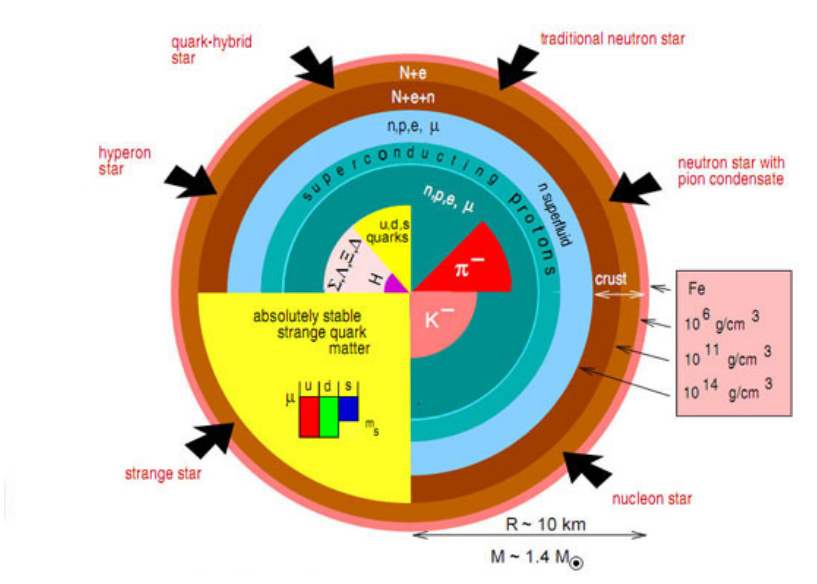
\includegraphics[scale=.42]{figures/RysEOS_examples.png}
            \caption{Przykładowe hipotetyczne modele budowy wnętrza gwiazdy neutronowej (Źródło: \textit{http://nrumiano.free.fr/Estars/neutrons.html}).}
            \label{RysEOS_examples}
        \end{figure}
        \section{Nierotujące gwiazdy neutronowe i kwarkowe}
        Gwiazdy neutronowe oraz kwarkowe są obiektami relatywistycznymi i do ich opisu należy posłużyć się Ogólną Teorią Względności. Dla statycznej, sferycznie symetrycznej gwiazdy pierwsze rozwiązania równań Einsteina pojawiły się w latach 30. i zostały nazwane równaniami Tolmana-Oppenheimera-Volkoffa (\citealp{Tolman1934}, \citealp{Tolman1939}, \citealp{Volkoff1939}), przedstawione poniżej jako równania \ref{EqTOV1} i \ref{EqTOV2}.
        \begin{equation}
            \frac{dP}{dr}=\frac{Gm\rho}{r^2}\left(1+\frac{P}{\rho c^2}\right)\left(1+\frac{4\pi Pr^3}{mc^2}\right)\left(1-\frac{2Gm}{rc^2}\right)^{-1}
            \label{EqTOV1}
        \end{equation}
        \begin{equation}
            \frac{dm}{dr}=4\pi r^2\rho
            \label{EqTOV2}
        \end{equation}
        \indent Zakładając pewną wartość gęstości w centrum gwiazdy $\rho_c$ oraz równanie stanu materii, a następnie rozwiązując równania Tolmana-Oppenheimera-Volkoffa (TOV) można wyznaczyć promień gwiazdy $R$ i jej masę $M$. Dla różnych równań stanu rozwiązanie równań TOV daje różne funkcje $M(R)$. Te zależności dla kilku przykładowych równań stanu przedstawia Rysunek \ref{RysEOS}. Dwie zielone linie symbolizują konfiguracje nierotujących gwiazd dziwnych, pozostałe linie zostały narysowane dla gwiazd neutronowych. Można zauważyć, że dla gwiazd neutronowych maksymalna masa osiągana jest dla konfiguracji o najmniejszym promieniu, tj. najbardziej skompresowanej. Z kolei zależności dla gwiazd kwarkowych wydają się być bardziej skomplikowane, a największa masa osiągana jest dla promienia bliskiego największemu promieniowi, jaki gwiazda może osiągnąć. Jednoczenie dla promienia odpowiadającego masie maksymalnej istnieje rozwiązanie o masie mniejszej o kilkadziesiąt procent.
        \begin{figure}[h!]
            \centering
            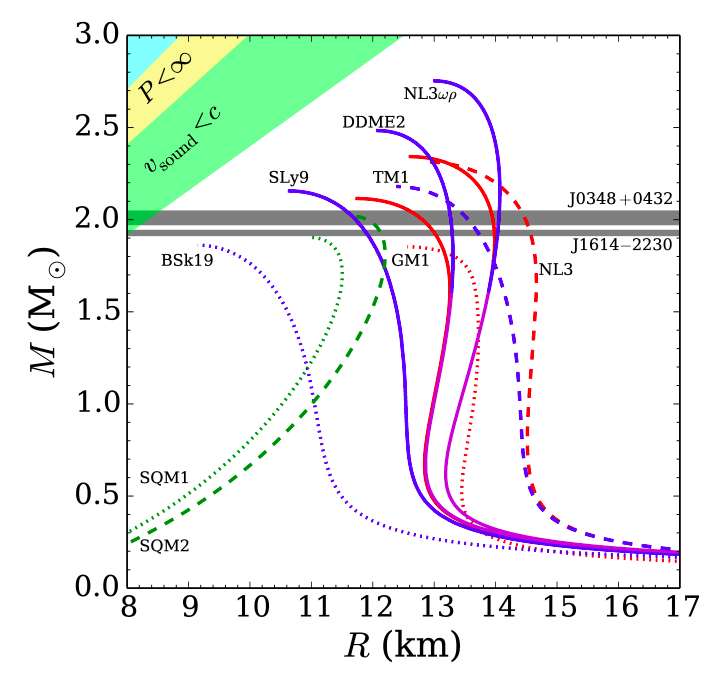
\includegraphics[scale=.31]{figures/RysEOS2.png}
            \caption{Zależności masy grawitacyjnej $M$ od promienia gwiazdy $R$ dla równań stanu gwiazd kwarkowych (linie zielone) oraz neutronowych (pozostałe linie) (Źródło: \citealp{Haensel2007}).}
            \label{RysEOS}
        \end{figure}\\
        \indent Okazuje się, że rozważając powyżej opisane obiekty jako sztywno rotujące, kształty funkcji $M(R)$ odtwarzają kształty ciągów konfiguracji statycznych. Jednak rotacja pozwala na osiąganie przez gwiazdy większych mas oraz promieni. Takie zjawiska mogą zachodzić np. w pulsarach, będących najliczniej obserwowanymi gwiazdami neutronowymi.
        \section{Wpływ rotacji na własności gwiazd zwartych}
        \subsection{Sztywna rotacja}
        Ciała rotujące sztywno charakteryzują się jednakową prędkością kątową w każdym ich punkcie, niezależnie od położenia. Przykładem ciała sztywno rotującego jest Ziemia, a dokładniej jej litosfera. W gwiazdach neutronowych to właśnie ten sposób rotacji jest najczęściej obserwowany, przede wszystkim w pulsarach. Modelowaniem gwiazd neutronowych sztywno rotujących o politropowym równaniu stanu zajmowali się m.in. \cite{Komatsu1989} i \cite{Cook1994a}. Z kolei dla tak samo rotujących gwiazd opisanych modelem worka badania przeprowadzili m.in. \cite{Gourgoulhon1999} i \cite{Stergioulas1999}.\\
        \indent Okazuje się, że dla sztywnej rotacji zarówno gwiazdy neutronowe jak i kwarkowe mogą osiągać większe masy niż te odpowiadające przypadkom nierotującym. Wynika to z faktu, iż powstająca w wyniku rotacji siła odśrodkowa wnosi dodatkowy wkład do rachunku sił w gwieździe i pozwala na zrównoważenie większej siły ciążenia. Ponadto, istnieją także stabilne konfiguracje rotujące, które nie posiadają swoich statycznych odpowiedników. Oznacza to, że gdyby taka konfiguracja zaczęła spowalniać, nie byłaby w stanie zmniejszyć swojej rotacji do zera, ponieważ zapadłaby się do czarnej dziury. Takie gwiazdy nazywane są supramasywnymi. Sztywna rotacja pozwala na osiąganie mas od $14\%$ do $22\%$ większych niż masy nierotujące dla gwiazd neutronowych (\citealp{Cook1994a}), a nawet do $44\%$ dla gwiazd dziwnych (\citealp{Rosinska2000}). Większy wzrost dla gwiazd kwarkowych wynika z faktu, iż poza siłą odśrodkową, ciśnieniem w gwieździe i działaniem grawitacji istnieje dodatkowa siła wiążąca kwarki, co pozwala na utrzymanie jeszcze wyższych prędkości rotacji. Ta własność może być kluczowa w rozstrzygnięciu czy gwiazdy kwarkowe istnieją - gdyby została zaobserwowana gwiazda o promieniu rzędu $10$ km i o prędkości rotacji większej niż jakakolwiek wartość przewidywana dla równań stanu gwiazd neutronowych, a jednak możliwej do osiągnięcia przez gwiazdę dziwną, byłaby to przesłanka potwierdzająca hipotezę o gwiazdach kwarkowych.\\
        \indent Zależności masy grawitacyjnej $M$ od promienia $R$ dla różnych konfiguracji przedstawia Rysunek \ref{RysMofR} -- lewy wykres przedstawia funkcję $M(R)$ dla gwiazdy neutronowej o równaniu stanu FPS (\citealp{Friedman1981}), po prawej przedstawiona jest ta sama zależność dla gwiazdy dziwnej opisanej modelem worka. Pogrubiona czarna linia to ciągi statycznych obiektów, cienkie czarne linie są konfiguracjami o ustalonej masie barionowej, coraz szybciej rotującymi im większa jest wartość promienia $R$. Prawostronną granicą dla tych ciągów są czerwone przerywane linie, symbolizujące konfiguracje keplerowskie. Limit keplerowski oznacza sytuację, w której siła odśrodkowa równoważy siłę grawitacji, a dalsze zwiększenie tempa rotacji skutkowałoby odpływem materii z równika gwiazdy. Niebieskie linie wyznaczają granicę, powyżej której nie istnieją ciągi o ustalonej masie barionowej posiadające odpowiednik nierotujący. Linie zielona i fioletowa to konfiguracje marginalnie stabilne względem osiowosymetrycznych zaburzeń.\\
        \begin{figure}[h!]
            \centering
            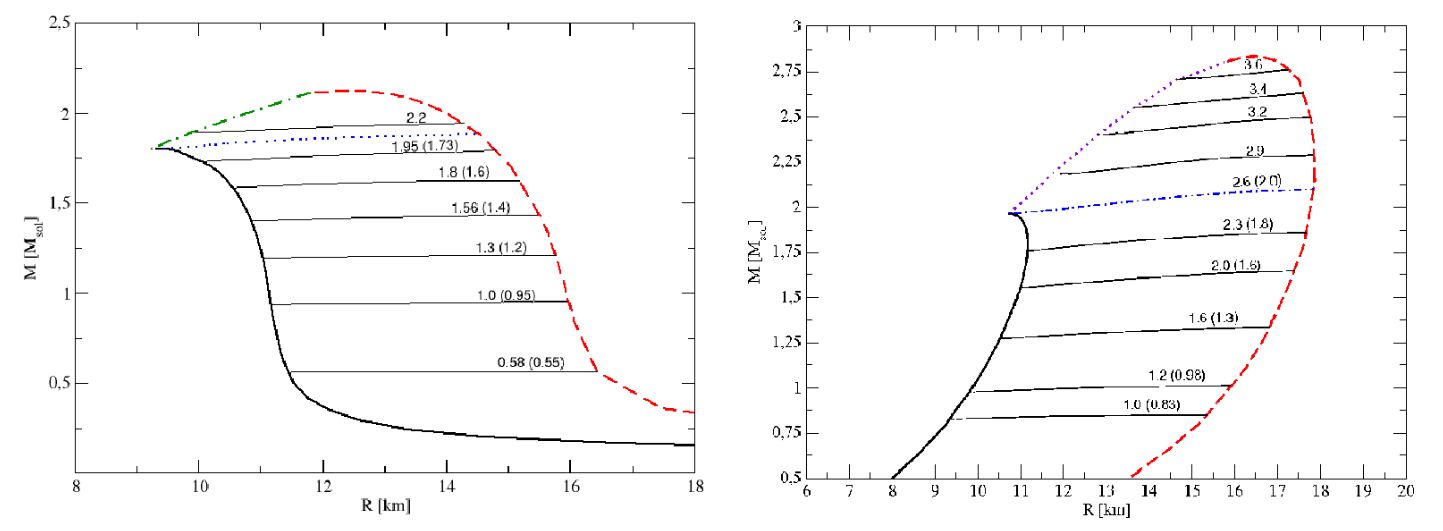
\includegraphics[scale=.28]{figures/RysMofR.png}
            \caption{Zależności masy $M$ od promienia gwiazdy $R$ o różnym tempie sztywnej rotacji dla ciągów gwiazd neutronowych opisanych równaniem stanu FPS (po lewej) oraz gwiazd kwarkowych opisanych modelem worka (po prawej). Pogrubione czarne linie odpowiadają przypadkom statycznym,  cienkie czarne linie to ciągi o ustalonej masie barionowej (w nawiasie), linie czerwone to konfiguracje na limicie keplerowskim, a linie zielona i fioletowa to gwiazdy marginalnie stabilne. Powyżej niebieskiej linii nie istnieją stabilne konfiguracje nierotujące. (Źródło: \citealp{Rosinska2007}).}
            \label{RysMofR}
        \end{figure}\\
        \indent Należy zauważyć, że w przypadku sztywnej rotacji największa masa $M_\textrm{max}$ zawsze osiągana jest dla konfiguracji keplerowskiej, która jest bliska konfiguracji rotującej najszybciej. Jednak dla bardziej zróżnicowanych profili rotacji gwiazdy jej masa może być jeszcze większa, limit keplerowski nie zawsze wiąże się z masą maksymalną, a przestrzeń rozwiązań jest bardziej zdywersyfikowana niż dla rotacji sztywnej, co zostanie przedstawione w kolejnym podrozdziale.
        \subsection{Różniczkowa rotacja}
        Rotacja różniczkowa, w przeciwieństwie do sztywnej, charakteryzuje się zależnością od położenia. Prędkość kątowa $\Omega$ zależy od współrzędnych astrograficznych $(r,\varphi,\theta)$, gwiazda może np. rotować szybciej na równiku niż w okolicach biegunów. Przykładami obiektów różniczkowo rotujących są Słońce, Jowisz, a także ziemska atmosfera. W przypadku gwiazd neutronowych takie zjawisko może zachodzić zaraz po ich utworzeniu w wyniku wybuchu supernowej albo jako produkt koalescencji dwóch gwiazd neutronowych. W wielu badaniach zakłada się, że prędkość kątowa takich obiektów zależy wyłącznie od odległości od osi rotacji $\varrho$.\\ \indent Najpowszechniej używanym (\citealp{Baumgarte2000}, \citealp{Lyford2003}, \citealp{Ansorg2009}) prawem rotacji jest prawo sformułowane przez \cite{Komatsu1989}:
        \begin{equation}
            F(\Omega)=A^2(\Omega_\textrm{c}-\Omega).
            \label{EqKomatsu}
        \end{equation}
        Wielkość $\Omega_\textrm{c}$ jest prędkością kątową w centrum gwiazdy, $\Omega$ to prędkość kątowa w wybranym punkcie, z kolei $A$ mówi o stopniu różniczkowej rotacji i wyrażana jest w jednostkach odległości. Mówi ona w jakiej odległości od osi rotacji wartość $\Omega$ spada o połowę względem $\Omega_\textrm{c}$. W celu ułatwienia obliczeń powszechnie stosuje się unormowaną wielkość $\tilde{A}=r_e/A$, gdzie $r_e$ oznacza promień gwiazdy na równiku. Im większa wartość $\tilde{A}$, tym bardziej stromy jest profil rotacji. Rysunek \ref{RysKomatsu} przedstawia profile rotacji dla dwóch stopni różniczkowej rotacji $\tilde{A}$.
       \begin{figure}[h!]
            \centering
            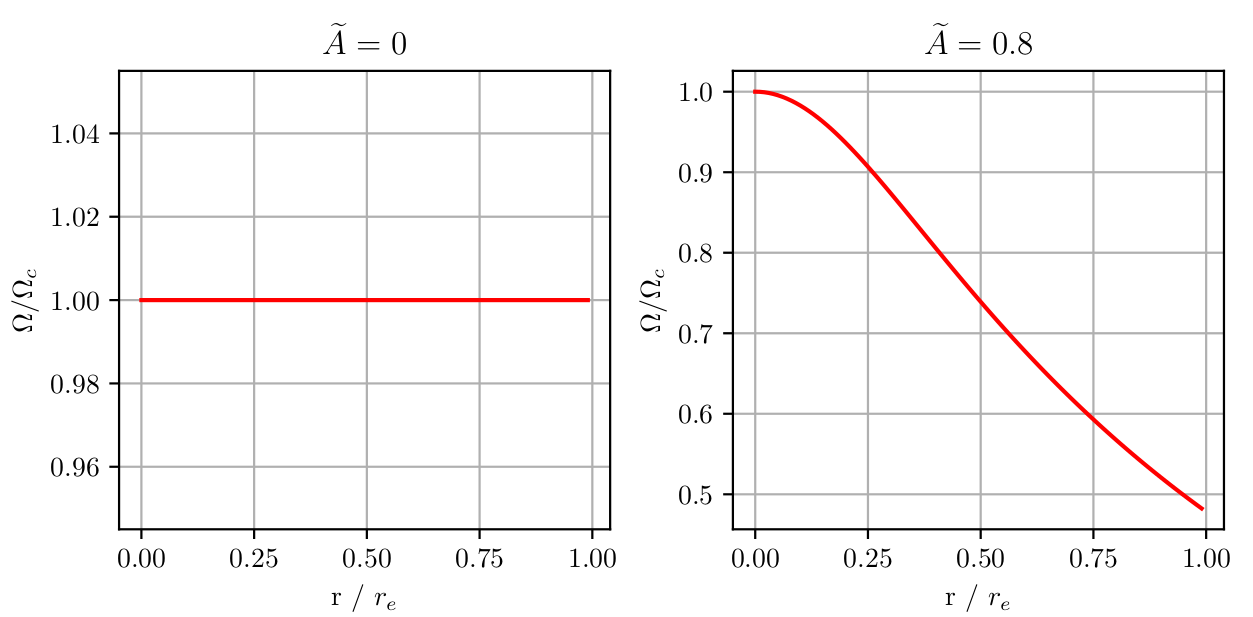
\includegraphics[scale=.3]{figures/RysKom.png}
            \caption{Profile różniczkowej rotacji dla ustalonych stopni różniczkowej rotacji $\tilde{A}=0$ i $\tilde{A}=0,8$. $\Omega$ to prędkość kątowa na danej odległości $r$ od osi rotacji,  $\Omega_\textrm{c}$ to prędkość kątowa w centrum gwiazdy.}
            \label{RysKomatsu}
        \end{figure}\\
        \indent W pracy \cite{Ansorg2009} wykazano istnienie czterech typów różniczkowo rotujących gwiazd opisanych równaniem stanu politropy, co okazało się prawdziwe również dla modelu worka (\citealp{Szkudlarek2019}). Gwiazdy należące do różnych typów przedstawia Rysunek \ref{RysTypy}. W ich opisie przydatny okazuje się być parametr $\tilde{\beta}$, który mówi o kształcie gwiazdy w okolicach równika i może przyjmować wartości z zakresu $[0,1]$. Dla gwiazdy ciągłej w środku o kształcie niemal toroidalnym (prawy dolny wykres na Rysunku \ref{RysKszt}) $\tilde{\beta}\rightarrow 1$; dla sfery $\tilde{\beta}=0,5$; dla konfiguracji na limicie keplerowskim $\tilde{\beta}\rightarrow 0$ (lewy górny wykres). Poszczególne typy istnieją tylko w określonych warunkach, co przedstawia Rysunek \ref{RysTypy}. Znajdują się na nim zależności $\tilde{\beta}(r_p/r_e)$ dla różnych stopni rotacji $\tilde{A}$. Istotna jest krytyczna wartość stopnia różniczkowej rotacji $\tilde{A}_{\textrm{crit}}$, która wydziela cztery charakterystyczne obszary. Można zauważyć, że typy zostały nazwane literami A, B, C, D i można je rozróżnić następująco -- ciągi konfiguracji o ustalonej wartości $\tilde{A}$ należą do typu:
        \begin{itemize}
            \item A, jeśli rozpoczynają jako konfiguracja statyczna, a kończą na limicie keplerowskim;
            \item B, jeśli osiągają zarówno konfigurację keplerowską, jak i kształty toroidalne;
            \item C, jeśli posiadają odpowiednik nierotujący (sferyczny), a także toroidalny;
            \item D, jeśli są ograniczone limitem keplerowskim z obu stron.
        \end{itemize}
        Należy zauważyć, że typy B i D nie posiadają żadnej konfiguracji statycznej i istnieją tylko w przypadkach, gdy gwiazda rotuje. Ponadto, dla rotacji sztywnej otrzymać można tylko typ A, z kolei pozostałe trzy istnieją wyłącznie wtedy, gdy gwiazda rotuje różniczkowo. Ważne jest także spostrzeżenie, że dla szybko rotujących gwiazd typu C największe gęstości nie znajdują się w ich centrum. Gdyby taka gwiazda jeszcze bardziej zwiększyła tempo rotacji, przyjęłaby kształt torusa -- możliwe, że taka konfiguracja pozwalałaby na osiągnięcie jeszcze większych mas, jednak takie hipotetyczne obiekty nie są rozważane.
         \begin{figure}[h!]
            \centering
            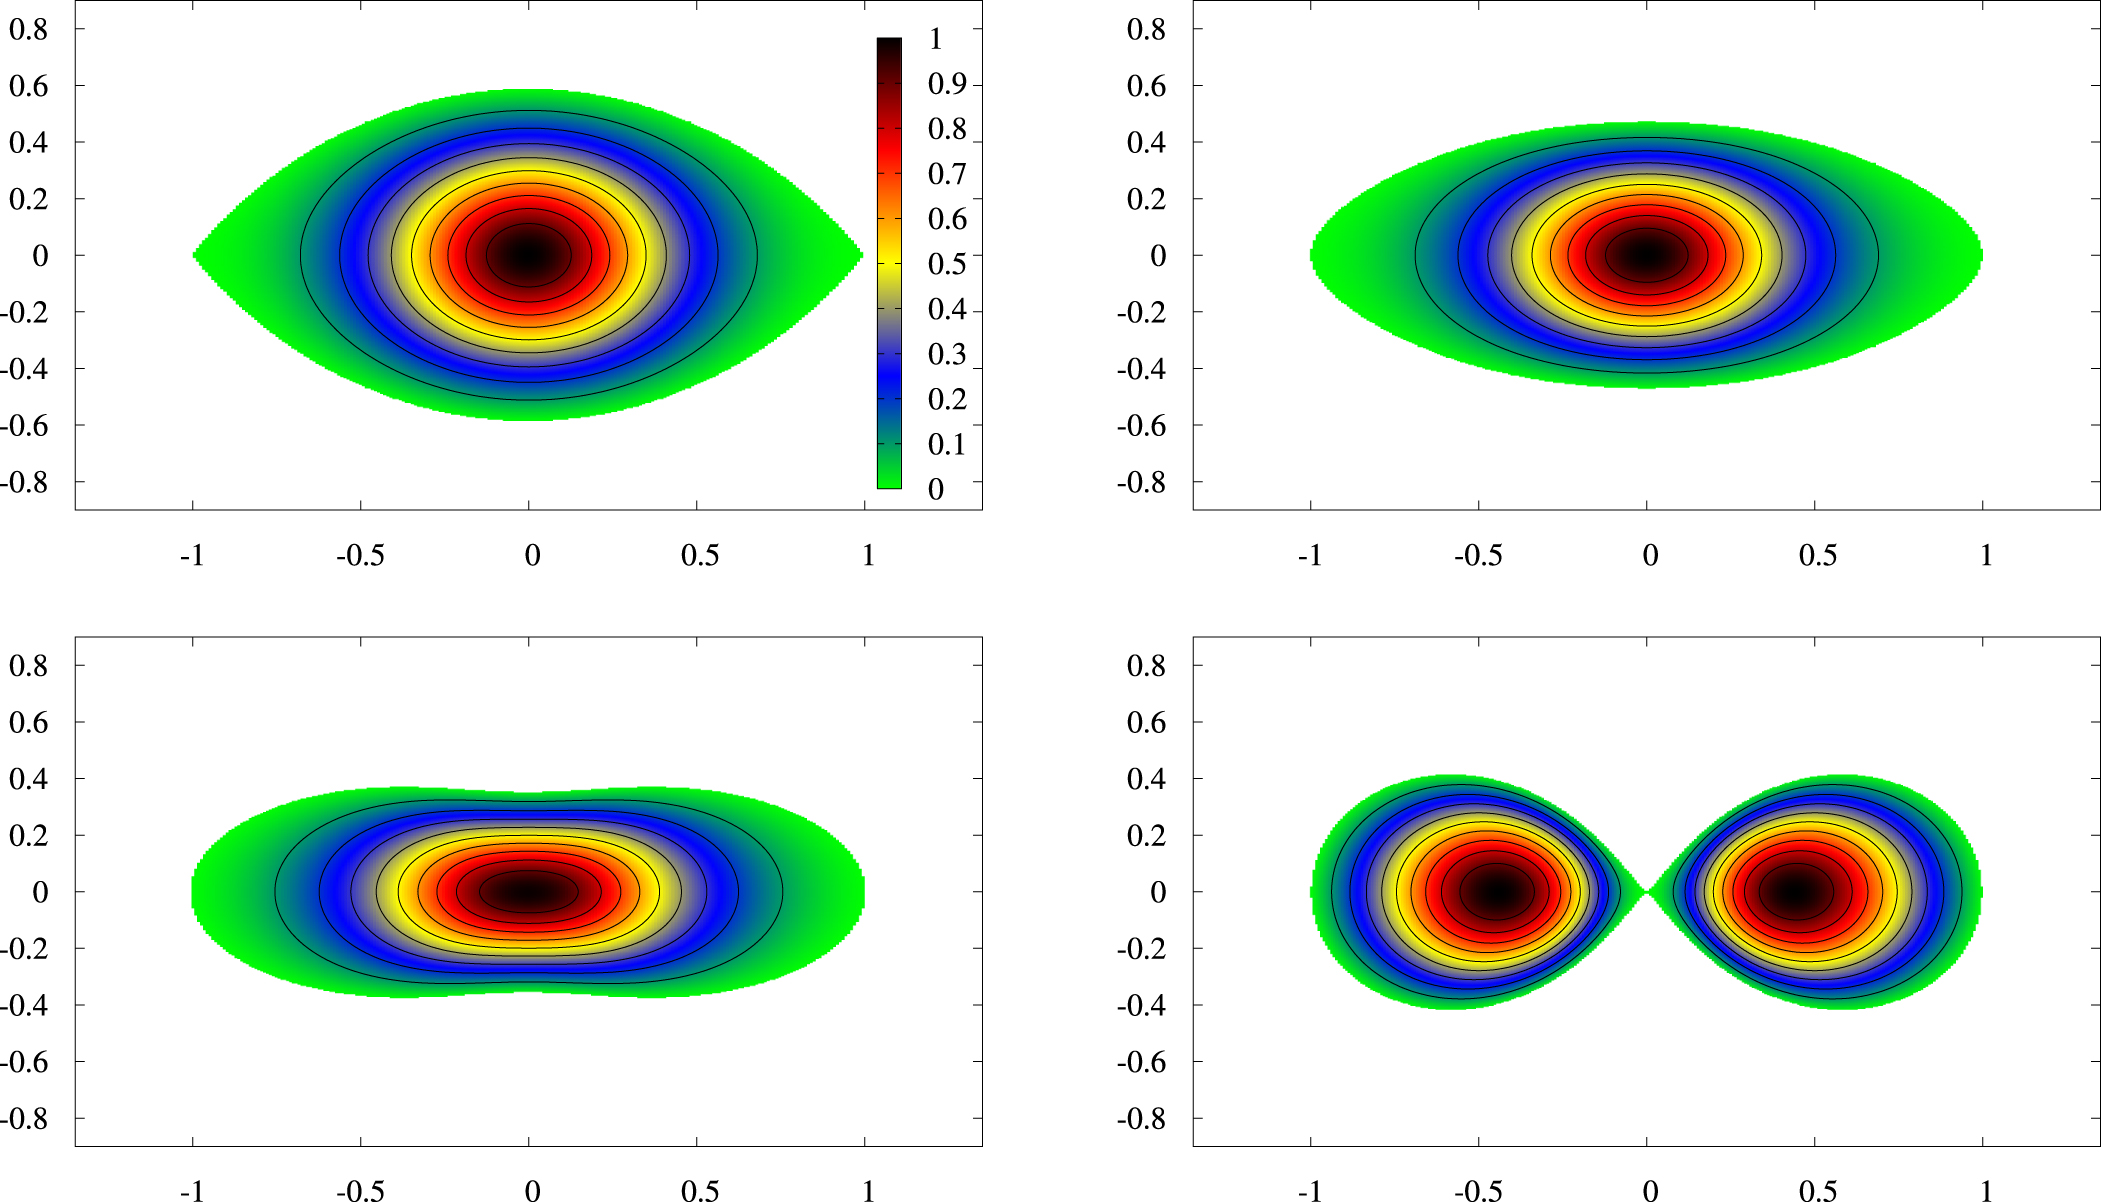
\includegraphics[scale=.6]{figures/RysKszt.jpg}
            \caption{Przykładowe przekroje gwiazd neutronowych rotujących różniczkowo: lewy górny wykres odpowiada gwieździe typu A sztywno rotującej ($\tilde{A}=0$) na limicie keplerowskim, prawy górny wykres to typ A o $\tilde{A}=0,5$, lewy dolny wykres to typ A o $\tilde{A}=0,7$, prawy dolny wykres to typ C, gdzie $\tilde{A}=1$. Izolinie odpowiadają stałej wartości gęstości. Dla prawej dolnej konfiguracji gęstość maksymalna nie znajduje się w centrum gwiazdy (Źródło: \citealp{Rosinska2017}).}
            \label{RysKszt}
        \end{figure}
        \begin{figure}[h!]
            \centering
            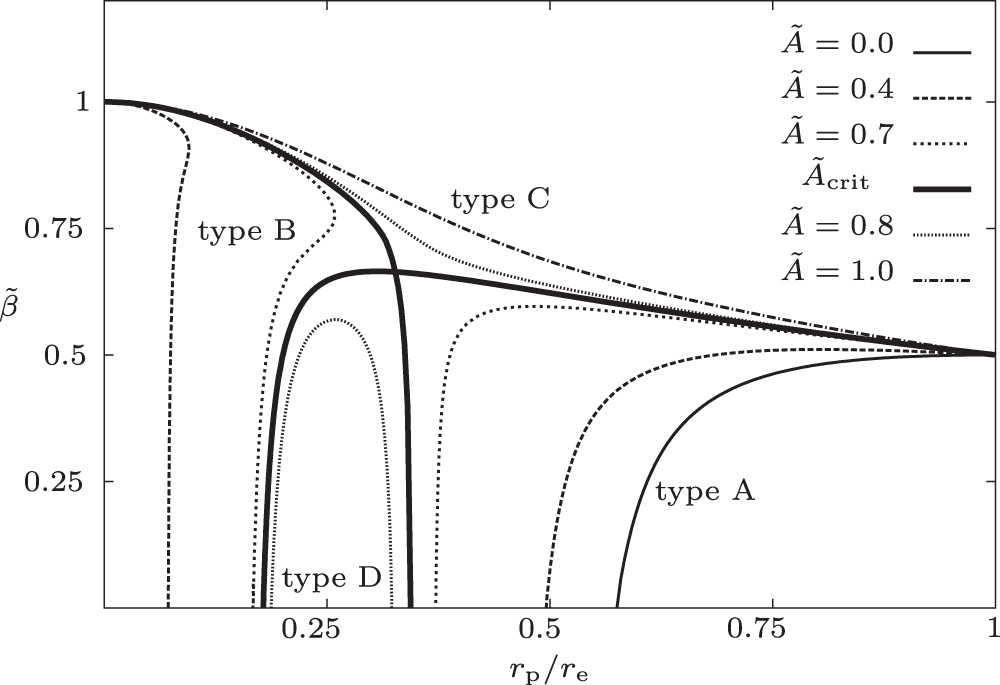
\includegraphics[scale=1.5]{figures/RysTypy.jpg}
            \caption{Zależności między parametrem $\beta$ a stosunkiem promieni biegunowego $r_p$ do równikowego $r_e$ dla politropowego równania stanu o wykładniku $\Gamma=2$ i ustalonych stopniach różniczkowej rotacji $\tilde{A}_{\textrm{crit}}$ (Źródło: \citealp{Ansorg2009}).}
            \label{RysTypy}
        \end{figure}
    \section{Wpływ rotacji na masę maksymalną}
        Rotacja gwiazdy wpływa na zakres mas, które może ona osiągać. Siła odśrodkowa pozwala na zrównoważenie większej siły grawitacji niż w przypadku, gdy obiekt jest statyczny. W przypadku sztywnej rotacji zachodzi prosta zależność -- im szybciej gwiazda rotuje, tym większe masy może posiadać. Górnym ograniczeniem jest w tym wypadku limit keplerowski, czyli sytuacja w której rotacja jest tak szybka, że doprowadza do odpływu materii z równika gwiazdy. Wykazano, że dla różnych równań stanu masa gwiazdy może wzrastać o $14-22 \%$ dla gwiazd neutronowych (\citealp{Cook1992}, \citealp{Cook1994a}, \citealp{Cook1994b}) oraz o $44\%$ w przypadku sztywno rotujących gwiazd dziwnych (\citealp{Rosinska2000}).
        \indent W przypadku różniczkowej rotacji maksymalne możliwe masy są zależne od typu, do którego należą (podrozdział 2.3.). Pierwsze badania gwiazd neutronowych różniczkowo rotujących dotyczyły typu A, u którego zaobserwowano wzrost maksymalnej masy $M_\textrm{max}$ wraz ze wzrostem stopnia różniczkowej rotacji $\tilde{A}$. Istnienie pozostałych typów nie zostało wtedy jeszcze przewidziane. W pracy \cite{Baumgarte2000} wykazano, że dla politropowego równania stanu o wykładniku $\Gamma=2$ masa może wzrosnąć nawet o $100\%$, co było kilkukrotnie większym wzrostem niż $14-22\%$ dla sztywnej rotacji.\\
        \indent Wraz z odkryciem istnienia różnych typów dla różniczkowej rotacji w gwiazdach neutronowych oraz wprowadzeniem tej klasyfikacji (\cite{Ansorg2009}) zauważono, że na wartości mas maksymalnych i m.in. zależność $M_\textrm{max}(\rho_\textrm{max})$ wpływa typ, do którego gwiazda należy. Jak można zauważyć na Rysunku \ref{RysMofE}, kształty obwiedni maksymalnych mas dla wartości $\epsilon_\textrm{max}$ z przedziału $[0;0,6]$ mogą się od siebie różnić, a także maksima tych funkcji mogą mieć różne wartości. Dla typu B można zaobserwować, że pozwala on na podtrzymanie dużo większych mas niż sztywna rotacja, a także różniczkowa rotacja dla typu A. Krytyczny stopnień różniczkowej rotacji wynosi w tym wypadku $\tilde{A}_\textrm{crit}=0,77$. Energia maksymalna w gwieździe $\epsilon_\textrm{max}$ jest odpowiednikiem $\rho_\textrm{max}$ i mówi on jak relatywistyczny jest rozpatrywany obiekt.
        \begin{figure}[h!]
            \centering
            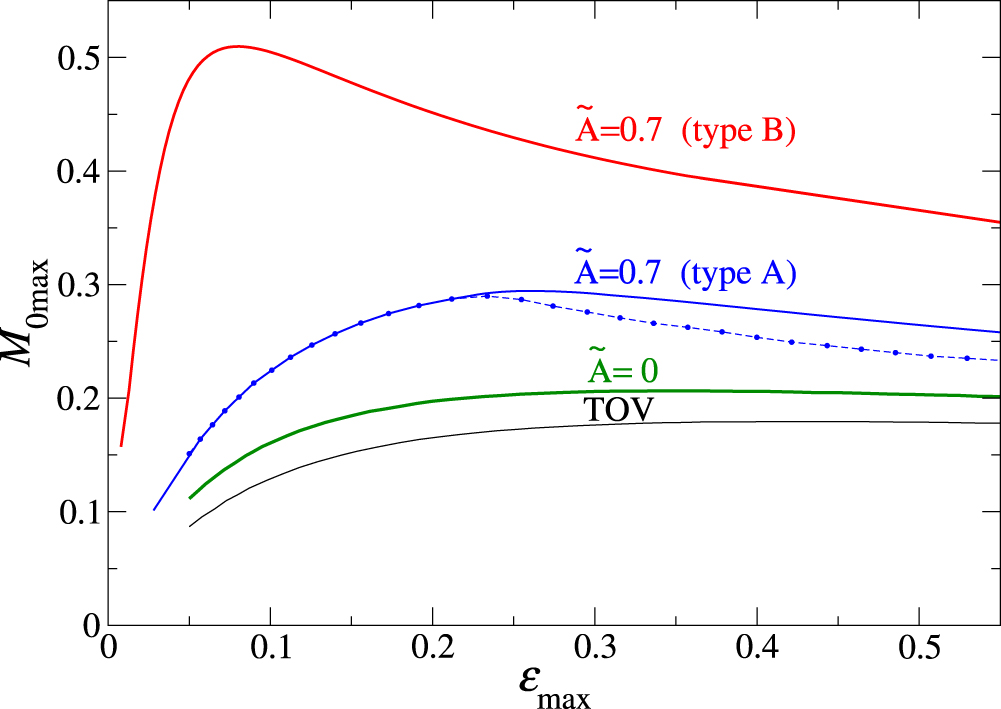
\includegraphics[scale=1.35]{figures/RysMofE.jpg}
            \caption{Zależności maksymalnej masy barionowej $M_{0\textrm{max}}$ od maksymalnej gęstości energii $\epsilon_\textrm{max}$ dla różniczkowo rotujących gwiazd neutronowych opisanych rownaniem stanu politropy o wykładniku $\Gamma=2$. Przedstawione ciągi odpowiadają konfiguracjom nierotującym (TOV), rotującym sztywno ($\tilde{A}=0$) oraz o stopniu różniczkowej rotacji $\tilde{A}=0,7$ dla typów A i B (Źrodło: \citealp{Rosinska2017}).}
            \label{RysMofE}
        \end{figure}\\
        \indent Uwzględniając wszystkie cztery typy, można zauważyć wyraźnie różne zależności $M_\textrm{max}(\tilde{A})$, gdzie $M_\textrm{max}$ jest masą maksymalną na całym rozpatrywanym przedziale maksymalnej gęstości energii $\epsilon_\textrm{max}$, określającej jak relatywistyczna jest gwiazda. Takie zależności przedstawia Rysunek \ref{RysMmaxofA}. Wyraźnie widać, że różniczkowa rotacja zwiększa $M_\textrm{max}$ tylko dla typu A. W typach B i C masa maksymalna maleje ze wzrostem stopnia różniczkowej rotacji, jednak jest ona zdecydowanie większa niż w typie A i pozwala na osiąganie mas nawet 4-krotnie większych niż masa konfiguracji statycznej. Dla typu D w tych badaniach nie wykonano wystarczającej ilości obliczeń, by przedstawić zależność od $\tilde{A}$. W poźniejszych pracach pokazano, że również dla typu D masa maksymalna $M_\textrm{max}$ maleje, gdy rośnie $\tilde{A}$.
        \begin{figure}[h!]
            \centering
            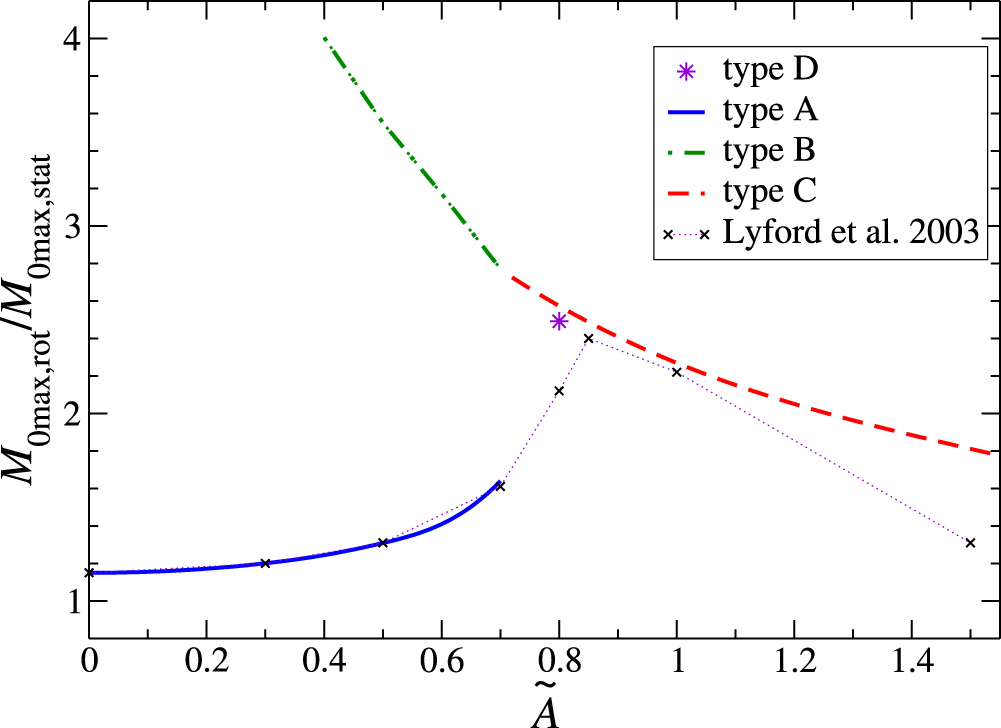
\includegraphics[scale=1.35]{figures/RysMmaxofA.jpg}
            \caption{Zależność maksymalnych względnych przyrostów masy barionowej gwiazd rotujących względem konfiguracji statycznej $M_{0\textrm{max,rot}}/M_{0\textrm{max,stat}}$ od stopnia różniczkowej rotacji $\tilde{A}$ dla wszystkich czterech typów. Na wykres zostały także naniesione wyniki otrzymane w pracy \cite{Lyford2003} (Źrodło: \citealp{Rosinska2017}).}
            \label{RysMmaxofA}
        \end{figure}\\
        Wspomniane badania dotyczyły równania stanu politropy o wykładniku politropy $\Gamma=2$. W pracy \cite{Studzinska2016} wykazano istnienie analogicznych zależności dla $\Gamma=1,5$ i $\Gamma=3$. Z kolei te zależności dla wykładników politropy $\Gamma\in\{1,8;2;2,5\}$ oraz równania stanu gwiazd dziwnych znaleziono w pracy \cite{Szkudlarek2019}, co przedstawia lewy panel Rysunku \ref{RysSzkEsp}. Prawy panel przedstawia zależności $M_\textrm{max}(\tilde{A})$ dla realistycznych równań stanu otrzymane przez \cite{Espino2019}.
        \begin{figure}[h!]
            \centering
            \begin{subfigure}{.5\textwidth}
              \centering
              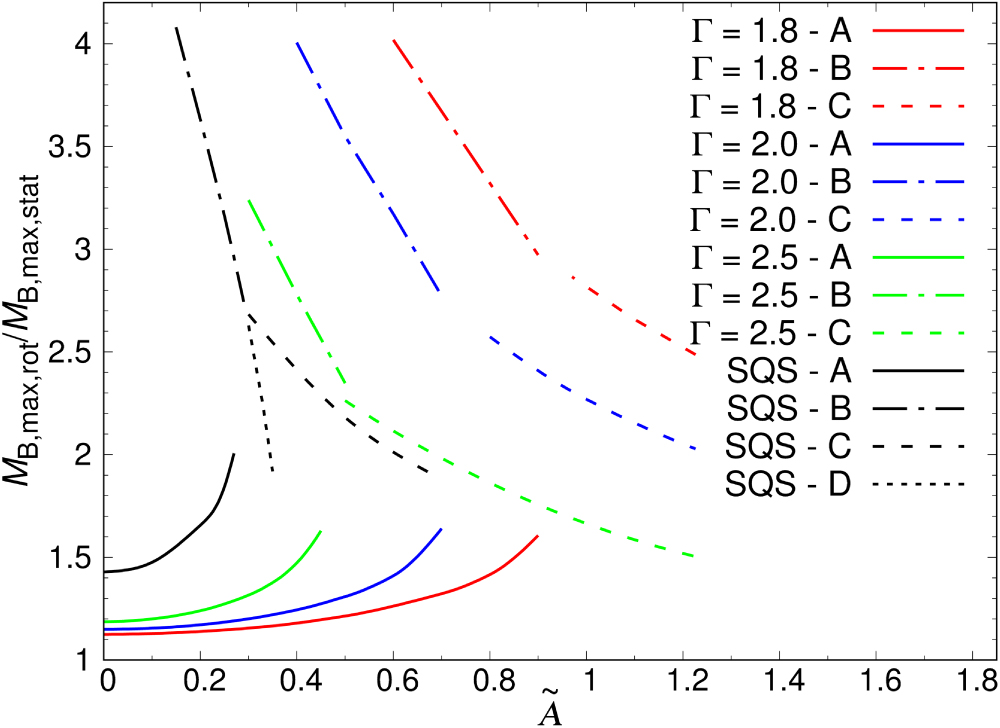
\includegraphics[width=.93\linewidth]{figures/RysSzk.jpg}
            \end{subfigure}%
            \begin{subfigure}{.5\textwidth}
              \centering
              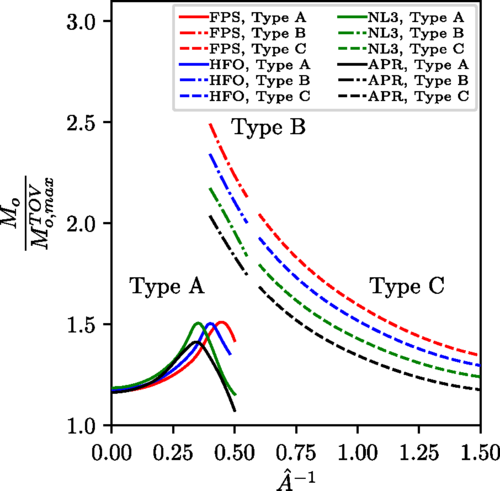
\includegraphics[width=.93\linewidth]{figures/RysEsp.png}
            \end{subfigure}
            \caption{Względne przyrosty barionowych mas maksymalnych $M_{0\textrm{max,rot}}/M_{0\textrm{max,stat}}$ w zależności od stopnia różniczkowej rotacji $\tilde{A}$ dla gwiazd neutronowych opisanych równaniem politropy o współczynnikach $\Gamma\in\{1,8;2;2,5\}$ i gwiazd dziwnych opisanych modelem worka (lewy wykres) oraz dla gwiazd neutronowych opisanych realistycznymi równaniami stanu FPS, HFO, NL3, APR (prawy wykres) (Źródła: \citealp{Szkudlarek2019}, \citealp{Espino2019}).}
            \label{RysSzkEsp}
        \end{figure}
    \section{Badanie stabilności różniczkowo rotujących gwiazd neutronowych i kwarkowych}
        Obecnie nie znaleziono kryterium stabilności gwiazd neutronowych rotujących różniczkowo, jednak dla sztywnej rotacji takie kryterium zostało opracowane przez \cite{Friedman1988}. Według niego statyczna konfiguracja najmasywniejsza jest także konfiguracją marginalnie stabilną. Dla jakiejkolwiek konfiguracji o większej gęstości centralnej $\rho_c$ gwiazda zapada się do czarnej dziury w dynamicznej skali czasowej. Dla sztywnej rotacji w punkcie marginalnie stabilnym osiągane jest także maksimum $M_0$ i minimum $J$.\\
        \indent Okazuje się, że dla małych stopni różniczkowej rotacji $\tilde{A}$ maksima mas ciągów o ustalonych momentach pędu $J$ zdają się dobrze wyznaczać konfiguracje marginalnie stabilne. Jednocześnie konstruując ciągi o ustalonej masie barionowej $M_0$ można zauważyć, że posiadają minima w niemal w tych samych punktach. Należy jednak podkreślić, że maksima dla $M_0=\textrm{const}$ i minima dla $J=\textrm{const}$ nie pokrywają się idealnie, są sobie równie jedynie w przybliżeniu. Ponadto dla coraz wyższych $\tilde{A}$ rzeczywista linia marginalnej stabilności skręca ku jeszcze mniejszym gęstościom niż te wyznaczone przez minima i maksima ciągów o ustalonych $J$ i $M_0$, nazywane po angielsku \textit{turning points}. Te zależności obrazuje Rysunek \ref{RysStab} -- czarne linie oznaczają ciąg konfiguracji statycznych oraz ciąg na limicie keplerowskim, kolorowe linie to ciągi o ustalonym momencie pędu, czarne kropki to \textit{turning points}, zielone kółka oznaczają konfiguracje stabilne, czerwone oznaczają gwiazdy dynamicznie niestabilne. Można zatem zauważyć, że dla różniczkowej rotacji kryterium Friedmana nie jest dokładne, jednak może być pierwszym przybliżeniem lokalizującym linię marginalnej stabilności. Według \cite{Giacomazzo2011} i \cite{Weih2018} nie wszystkie konfiguracje na lewo od linii maksimów dla $J=\textrm{const}$ są stabilne, ale za to wszystkie konfiguracje dla większych $\rho_c$ są niestabilne. \\
        \indent Położenie linii marginalnej stabilności na wykresie $M(\rho_\textrm{c})$ przedstawia Rysunek \ref{RysTak}.  Czarne ciągłe linie oznaczają odpowiednio ciąg konfiguracji statycznych i limit keplerowski. Rysunek ten dotyczy sztywnej rotacji, zatem limit keplerowski oznacza także maksimum masy dla określonego $\rho_\textrm{c}$. Czarnymi wypełnionymi kropkami zaznaczone są maksima tych ciągów na całym rozpatrywanym przedziale $\rho_\textrm{c}$. Można zauważyć, że linia marginalnej stabilności przebiega po prawej stronie względem maksimum limitu keplerowskiego. Oznacza to, że przyjmując linię minimów dla $M_0=\textrm{const}$ lub maksimów przy $J=\textrm{const}$ jako kryterium stabilności gwiazd neutronowych różniczkowo rotujących, konfiguracje najmasywniejsze mogą okazać się stabilne względem zapadania do czarnej dziury.
        \begin{figure}[h!]
            \centering
            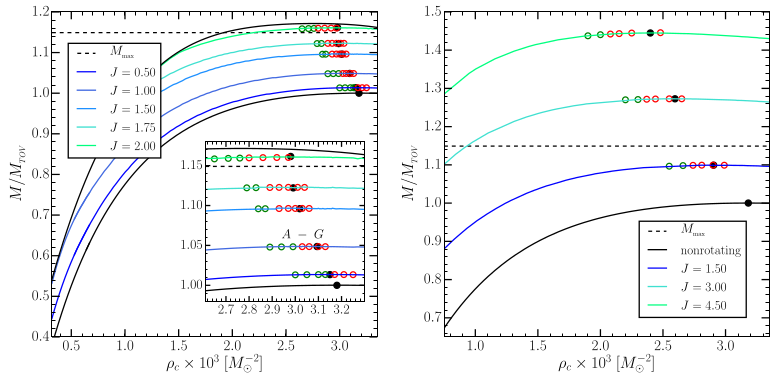
\includegraphics[scale=.52]{figures/RysStab.png}
            \caption{Ciągi konfiguracji gwiazd neutronowych o ustalonym momencie pędu dla dwóch stopni różniczkowej rotacji $\tilde{A}=0,2$ (typ A) i $\tilde{A}=0,77$ (typ C). Czarne linie oznaczają konfigurację statyczną oraz limit keplerowski (dla typu C limit keplerowski nie istnieje). Czarne kropki symbolizują maksima ciągów, dla konfiguracji zaznaczonych kolorowymi kółkami zostaly przeprowadzone obliczenia hydrodynamiczne -- kolor zielony oznacza stabilną konfigurację, a czerwony niestabilną (Źrodło: \citealp{Weih2018}).}
            \label{RysStab}
        \end{figure}
        \begin{figure}[h!]
            \centering
            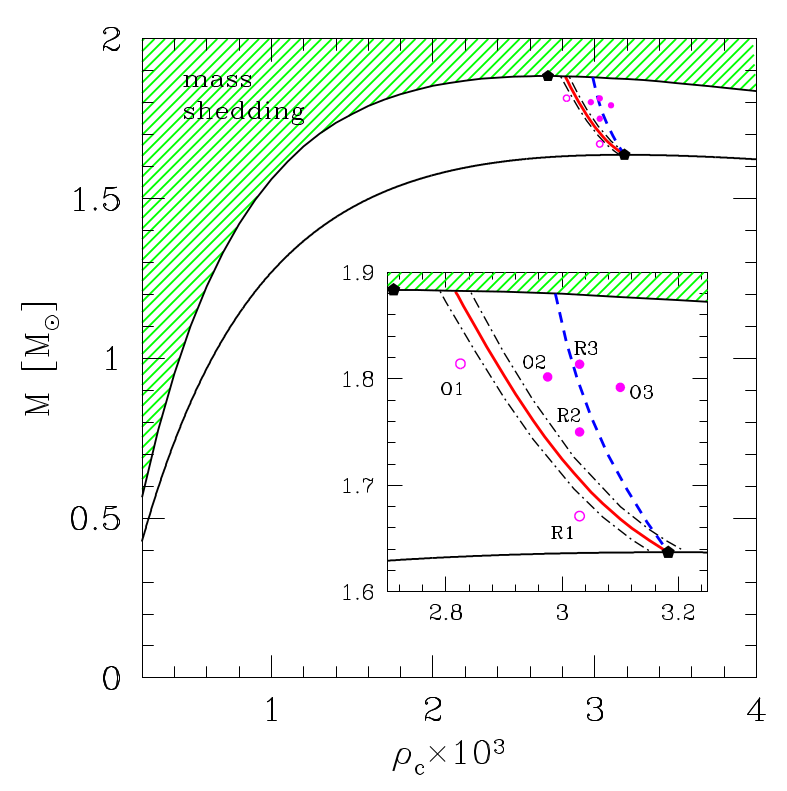
\includegraphics[scale=.3]{figures/RysTak.png}
            \caption{Zależności mas $M$ od gęstości centralnych $\rho_\textrm{c}$. Czarne linie odpowiadają konfiguracjom nierotującym (dolna linia) i konfiguracjom rotującym na limicie keplerowskim (górna linia). Powyżej limitu keplerowskiego zachodzi odpływ masy (ang. \textit{mass shedding}). Czarne punkty to maksima ciągów statycznego i keplerowskiego. Niebieska przerywana linia została wyznaczona przez \textit{turning points}. Puste kółka oznaczają konfiguracje niestabilne w dynamicznej skali czasowej, wypełnione kółka to konfiguracje stabilne. Jak zostało już wspomniane, rzeczywista linia marginalnej stabilności jest przesunięta ku mniejszym $\rho_\textrm{c}$ -- symbolizuje ją czerwona ciągła linia (Źródło: \citealp{Takami2011}).}
            \label{RysTak}
        \end{figure}
    \section{Uniwersalne relacje pomiędzy masą a momentem pędu}
        Omawiane w poprzednim podrozdziale konfiguracje marginalnie stabilne charakteryzują się osiągnięciem maksimum masy grawitacyjnej $M$ dla ustalonej masy barionowej $M_0$. W dalszej części tej pracy takie przypadki będą nazywane marginalnie stabilnymi, bądź krytycznymi. W pracach \cite{Bozzola2018} i \cite{Weih2018} zauważono istnienie pewnych relacji pomiędzy krytyczną masą grawitacyjną $M$, krytyczną masą barionową $M_0$ i odpowiadającym im momentem pędu $J$. Ponadto, okazały się one być uniwersalne dla różnych stopni różniczkowej rotacji, typu gwiazdy i równania stanu. Relację $M(J)$ według \cite{Bozzola2018} można przybliżyć funkcją:
        \begin{equation}
            \frac{M}{M^*}=1+0,29\left(\frac{cJ}{GM^{*^2}}\right)^2-0,10\left(\frac{cJ}{GM^{*^2}}\right)^4,
            \label{EqUnNeu}
        \end{equation}
        gdzie $M^*$ jest masą maksymalną dla konfiguracji nierotujących, $c$ to prędkość światła, a $G$ to stała grawitacji. Wymienione trzy wielkości służą do normalizacji $M$ i $J$. Dopasowanie funkcji do danych przedstawia lewy panel Rysunku \ref{RysUni}, gdzie kolorowe punkty oznaczają konfiguracje marginalnie stabilne dla różnych równań stanu. Z kolei po prawej stronie można zauważyć analogicznie dobraną relację $M_0(J)$ i pasujące do niej dane uzyskane dla dwóch politropowych równań stanu o różnych wykładnikach $\Gamma=1+1/n$. Poza nimi, naniesione zostały także punkty krytyczne dla gwiazd opisanych modelem worka (różowe kwadraty), które w przeciwieństwie do wszystkich innych zbadanych równań okazują się nie spełniać zaproponowanej relacji. Jednak również punkty dla gwiazd dziwnych wydają się leżeć na jednej krzywej, która została przybliżona jako:
        \begin{equation}
            \frac{M_0}{M_0^*}=1+0,87\left(\frac{cJ}{GM_0^{*^2}}\right)^2-0,6\left(\frac{cJ}{GM_0^{*^2}}\right)^4.
            \label{EqUnSQS}
        \end{equation}
        \begin{figure}[h!]
            \centering
            \begin{subfigure}{.5\textwidth}
              \centering
              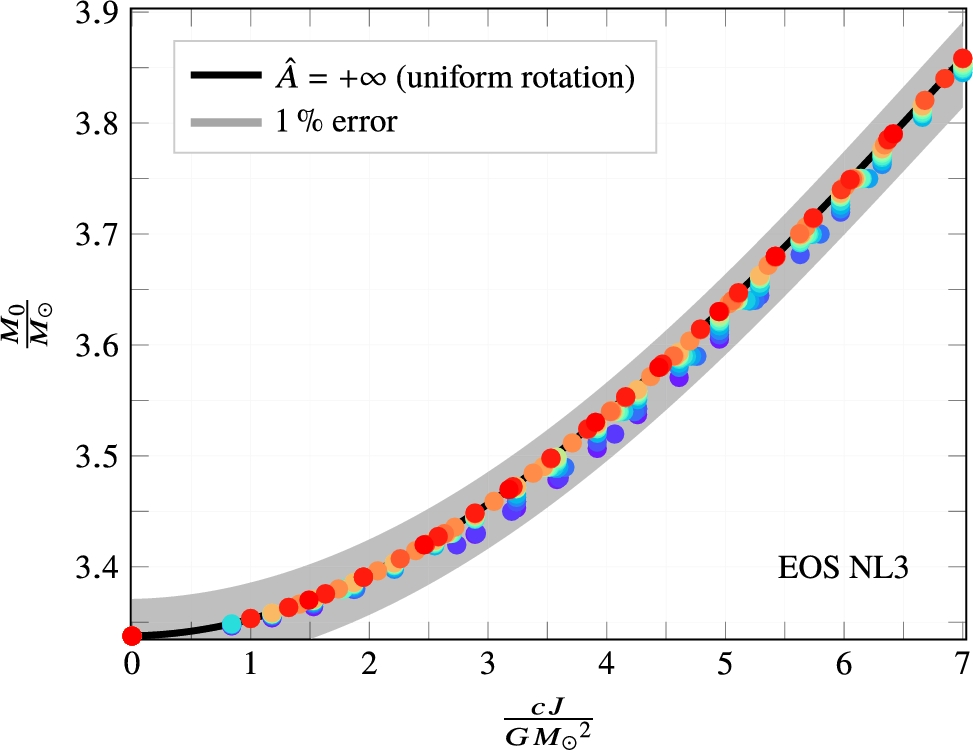
\includegraphics[width=.98\linewidth]{figures/RysUni1.jpeg}
            \end{subfigure}%
            \begin{subfigure}{.5\textwidth}
              \centering
              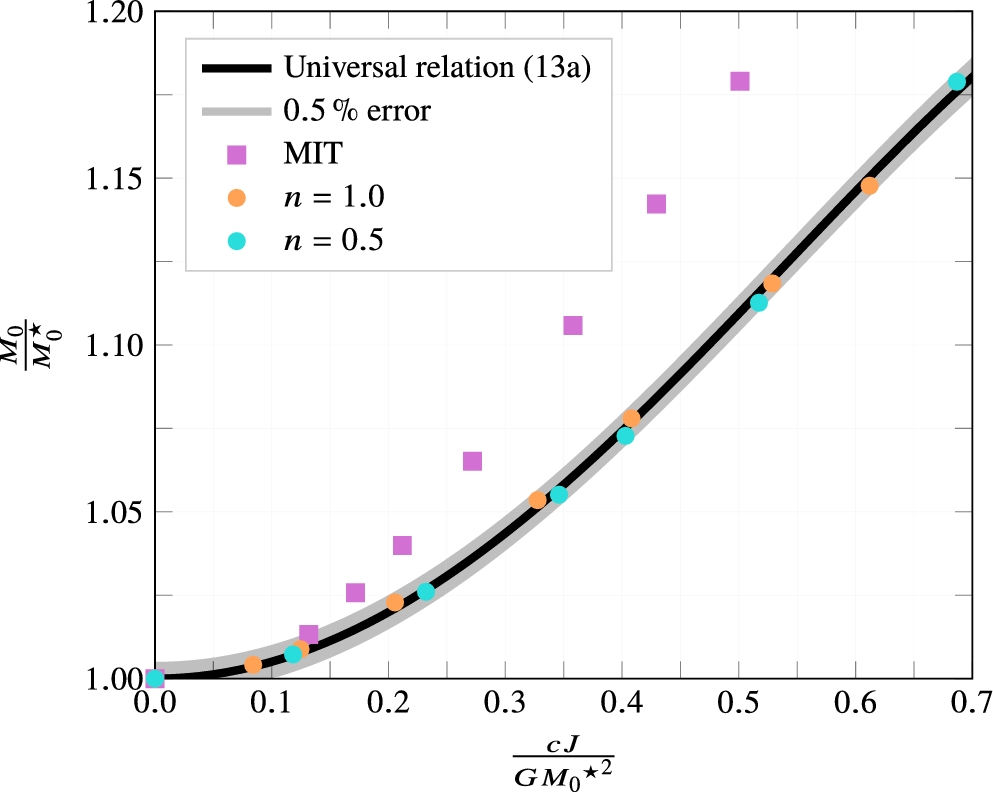
\includegraphics[width=.98\linewidth]{figures/RysUni2.jpeg}
            \end{subfigure}
            \caption{Wykresy zależności $M(J)$ (lewy panel) i $M_0(J)$ (prawy panel) oraz punkty krytyczne dla różnych równań stanu gwiazd neutronowych, oznaczone jako kolorowe kropki. Różowe kwadraty oznaczają punkty marginalnej stabilności dla modelu worka \textit{MIT bag model} (Źródło: \cite{Bozzola2018}).}
            \label{RysUni}
        \end{figure}
    \chapter{Metodologia}
        \section{Kod FlatStar}
        W celu zbadania własności gwiazd neutronowych i dziwnych użyty został kod numeryczny FlatStar (\cite{Ansorg2009}). Jest to kod w pełni relatywistyczny, oparty na metodzie pseudospektralnej (\citealp{Bonazzola1993}). Umożliwia obliczanie stacjonarnych gwiazd osiowosymetrycznych, z możliwością modyfikowania m.in. prawa rotacji czy równania stanu, co zostało wykorzystane poprzez wprowadzenie na potrzeby mojej pracy politropowego równania stanu gwiazd neutronowych o wykładniku $\Gamma=2$ oraz modelu worka. Kod pozwala na bardzo dokładne obliczenia, ograniczone przede wszystkim wewnętrzną dokładnością numeryczną maszyny obliczeniowej. Dzięki temu możliwe jest szczegółowe badanie przestrzeni rozwiązań dla gwiazd neutronowych rotujących różniczkowo nawet w ekstremalnych przypadkach, takich jak konfiguracja przedstawiona na rysunku \ref{RysKot}. Jest to gwiazda wysoce relatywistyczna o $\textrm{log}H_{\textrm{max}}=0.6$, wysokim stopniu różniczkowej rotacji $\tilde{A}=0.9$ i wyjątkowo spłaszczona, tj. o stosunku promienia polarnego do równikowego $r_p/r_e=0.005$. Poniższa konfiguracja jest toroidalna, a jednocześnie bliska limitu keplerowskiego, co jest dużym wyzwaniem numerycznym. Kod FlatStar jest jedynym kodem, przy pomocy którego mogą być modelowane rotujące gwiazdy w całej przestrzeni rozwiązań.
        \begin{figure}[h!]
            \centering
            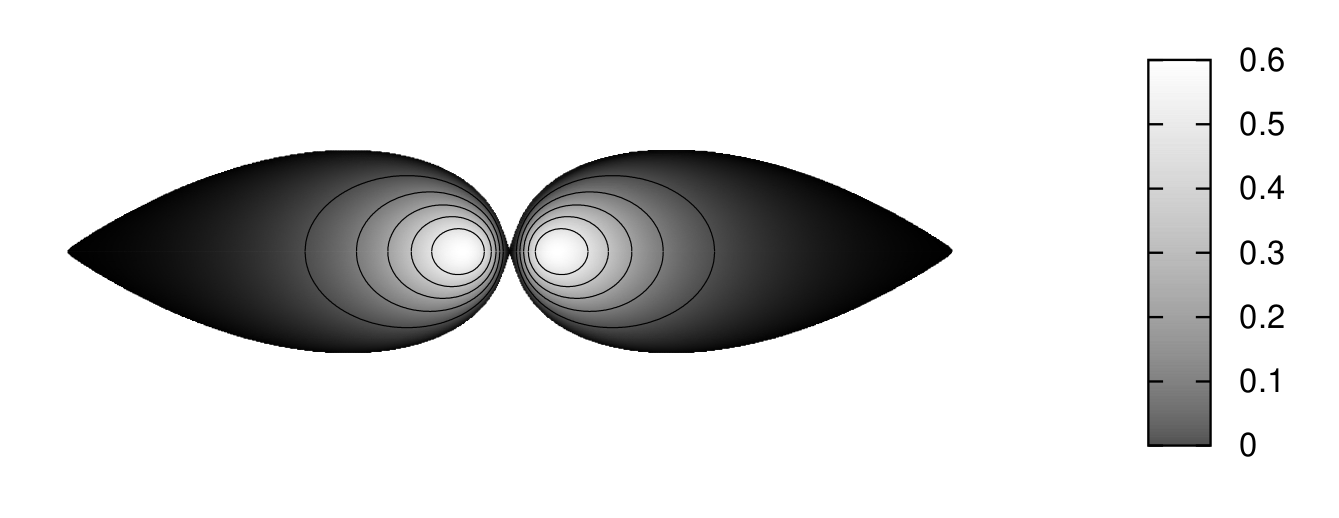
\includegraphics[scale=.33]{figures/RysKot.png}
            \caption{Przykład ekstremalnego modelu różniczkowo rotującej gwiazdy neutronowej o kształcie toroidalnym na limicie keplerowskim o parametrach $\textrm{log}H_{max}=0.6$, $\tilde{A}=0.9$ oraz $r_p/r_e=0.005$ (Źródło: \citealp{Ansorg2009}).}
            \label{RysKot}
        \end{figure}\\
        \indent W kodzie FlatStar wprowadzane są dwie domeny -- wewnętrzna obejmuje całą gwiazdę, zewnętrzna opisuje otoczenie obiektu. Granica między domenami została wybrana jako wspólna z powierzchnią gwiazdy. Wewnątrz domen znajdują się siatki punktów opisujących gwiazdę. Dla każdego z punktów wyznaczane są charakterystyczne parametry, co prowadzi do układu równań. Równania rozwiązywane są metodą Newtona-Raphsona, nazywaną także metodą stycznych. Przykładowe mapowanie przedstawia rysunek \ref{RysMap}.
        \begin{figure}[h!]
            \centering
            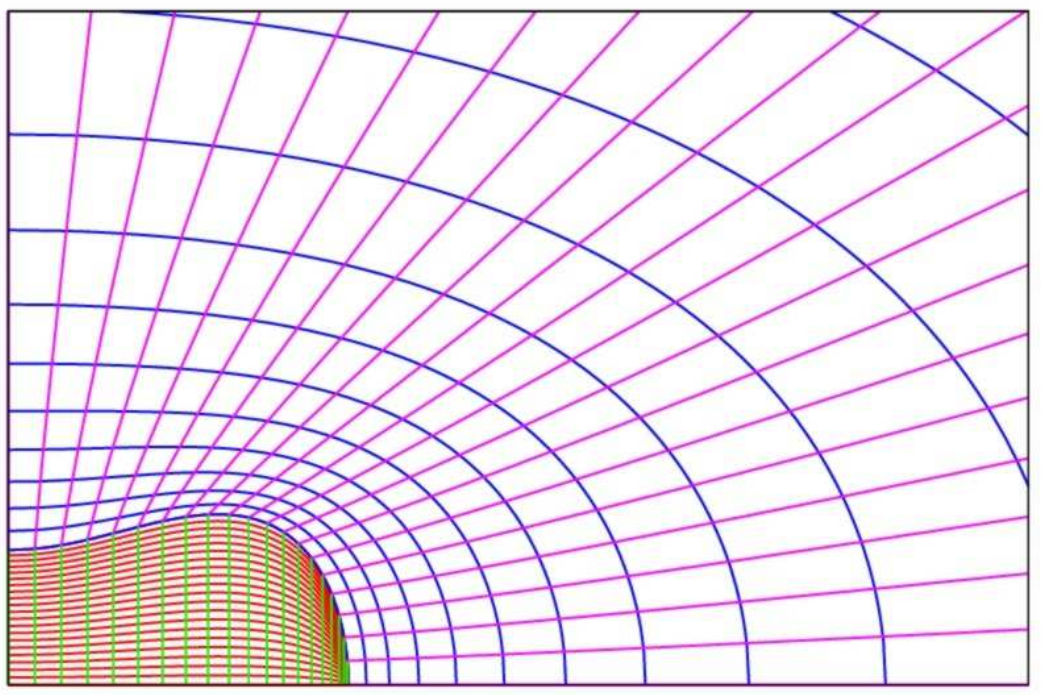
\includegraphics[scale=.27]{figures/RysMap.png}
            \caption{Przykładowy dwudomenowy podział gwiazdy wraz z siatkami punktów (Źródło: \citealp{Rosinska2017}).}
            \label{RysMap}
        \end{figure}\\
        \indent Dla każdej obliczanej konfiguracji kod zwraca parametry gwiazdy, m.in. $\tilde{\beta}$, $r_p/r_e$, $\tilde{A}$, $H_{\textrm{max}}$, $H\textrm{c}$, $J$, $M$, $M_0$ (te wielkości zostaną omówione w kolejnym podrozdziale). Na wejściu przyjmowane są trzy wybrane parametry oraz informacje na temat pierwszej konfiguracji gwiazdowej. Kod oblicza ciągi konfiguracji od pierwszej konfiguracji do konfiguracji opisanej trzema docelowymi parametrami. Częstą praktyką jest wprowadzenie dwóch wielkości identycznych jak dla przypadku startowego i badanie właściwości gwiazd względem zmienności jednego z parametrów.\\
        \indent W kodzie FlatStar jednostki są znormalizowane, tzn. $c=G=1$.
        \section{Najważniejsze parametry}
        W tym podrozdziale zostaną przypomniane bądź zdefiniowane najważniejsze parametry, które zostały użyte w obliczeniach wykonanych na potrzeby tej pracy. Jednym z takich parametrów jest $\tilde{\beta}$, który określa kształt gwiazdy w okolicach jej równika. Dla konfiguracji ze szpicami na równiku $\tilde{\beta}\rightarrow 0$. Gdy obiekt przechodzi do konfiguracji toroidalnych, okolice równika są niemal pionowe i wtedy $\tilde{\beta}\rightarrow 1$.  Takie przypadki to odpowiednio lewy górny i prawy dolny panel na Rysunku \ref{RysKszt}.\\
        \indent Drugim istotnym parametrem jest stosunek promienia polarnego do równikowego $r_p/r_e$. Ponieważ rotacja może jedynie spłaszczać gwiazdę, a nie wydłużać, zakres przyjmowanych wartości wynosi $[0,1]$.\\
        \indent Kolejną ważną wielkością jest $\tilde{A}$, która określa stopień różniczkowej rotacji w gwieździe. Im większa $\tilde{A}$, tym bardziej stromy jest profil rotacji, co pokazuje Rysunek \ref{RysKomatsu}. Za pomocą wymienionych trzech parametrów $(\tilde{\beta},r_p/r_e,\tilde{A})$ można jednoznacznie określić do którego typu (podrozdział 2.3.3.) należy badana gwiazda.\\
        \indent Wcześniej przytaczana juz była gęstość maksymalna $\rho_{\textrm{max}}$, dla większości konfiguracji znajdująca się w centrum gwiazdy. Można zauważyć, że im szybciej gwiazda rotuje, tym większa jest wartość $\rho_{\textrm{max}}$. Zatem ten parametr pozwala określić jak bardzo relatywistyczny jest obiekt. Analogiczną wielkością do $\rho$ jest entalpia relatywistyczna $H$, zdefiniowana w następujący sposób:
        \begin{equation}
            H(P)=\int_0^P \frac{dP}{\epsilon(P)+P}.
        \end{equation}
        $P$ oznacza ciśnienie w gwieździe, $c$ jest prędkością światła, z kolei gęstość energii $\epsilon(p)$ jest określona równaniem stanu, np. dla politropy $\epsilon(P)=P+\sqrt{p/K}$, gdzie $K$ to stała politropy. Istotną zaletą relatywistycznej entalpii $H$ jest to, że jest bezwymiarowa. Jak można się domyśleć, analogicznym do $\rho_{\textrm{max}}$ parametrem jest $H_{\textrm{max}}$ i to właśnie ojego będę używał w analizie obliczeń. Ponieważ istotne w analizie wyników dla gwiazd typu C jest przejście do konfiguracji toroidalnych, przytaczana będzie także wielkość $H_\textrm{c}$, będąca entalpią w centrum gwiazdy.\\
        \indent Poza powyższymi, przydatne w dalszym opisie własności gwiazd różniczkowo rotujących będą moment pędu gwiazdy $J$, masa grawitacyjna $M$ oraz masa barionowa $M_0$. Masa barionowa nazywana jest także masą spoczynkową, ponieważ jest sumą mas spoczynkowych wszystkich barionów w gwieździe. Jest ona niezmienna względem tempa rotacji gwiazdy. Z kolei na masę grawitacyjną wpływają efekty relatywistyczne, tj. im szybciej rotuje gwiazda, tym większa staje się $M$, za to $M_0$ pozostaje stała.
        \section{Metodologia obliczeń}
            W ramach tej pracy wykonałem obliczenia dla gwiazd opisanych równaniem stanu politropy o wykładniku $\Gamma=2$ oraz jednym z modeli worka \textit{MIT Bag model}. Pierwsze zostały obliczone ciągi gwiazd statycznych oraz sztywno rotujących ($\tilde{A}=0$) dla $H_\textrm{max}\in [0,05;0,6]$. \\
            \indent Późniejsze obliczenia dotyczyły gwiazd neutronowych o stopniach różniczkowej rotacji $\tilde{A}=0,7$ i $1,0$ oraz kwarkowych dla $\tilde{A}=0,2$; $0,25$; $0,3$ i $0,5$. W przypadkach konfiguracji typu A wyznaczono ich limity keplerowskie oraz ciągi mas maksymalnych (typ A osiąga maksimum masy zaraz przed limitem keplerowskim), dla typu C wyznaczono suprema masy, czyli konfiguracje o $r_p/r_e\rightarrow 0$. Znalazłem także gwiazdy bliskie przejścia do konfiguracji toroidalnych, gdzie $H_\textrm{max}\neq H_\textrm{c}$. Następnie wykonałem obliczenia dla ciągów o ustalonej masie barionowej $M_0$ w celu znalezienia minimów masy grawitacyjnej $M$. Wyznaczyłem oszacowane linie marginalnej stabilności za pomocą wspomnianych minimów, czyli punktów krytycznych. Znalezione zostały także maksima mas na całym badanym przedziale $H_\textrm{max}$ dla przypadków statycznych, sztywnej rotacji, limitów keplerowskich oraz ciągów najmasywniejszych.\\
            \indent Następnie zbadane zostały zależności \ref{EqUnNeu} i \ref{EqUnSQS} i ich dopasowanie do znalezionych wcześniej punktów krytycznych. Zostały one wyznaczone dla małych wartości momentów pędu $J$ oraz mniejszych mas $M$ i $M_0$.  Korzystając z obliczonych wcześniej konfiguracji krytycznych dla szerokiego zakresu mas i momentów pędu zaproponowałem nowe funkcje $M(J)$ dla gwiazd neutronowych i $M_0(J)$ dla gwiazd kwarkowych. Pokazałem, że istnieją podobne zależności również dla modeli toroidalnych.
    \chapter{Wyniki}
        \section{Przestrzeń rozwiązań dla różniczkowo rotujących gwiazd zwartych}
        \subsection{Gwiazdy neutronowe}
            W ramach tej pracy wykonane zostały obliczenia takich parametrów jak masa grawitacyjna $M$, masa barionowa $M_0$, promień gwiazdy $R$, moment pędu $J$ czy maksymalna entalpia relatywistyczna $H_\textrm{max}$ dla gwiazd neutronowych opisanych politropowym równaniem stanu. Rysunek \ref{RysMofHpolA07} przestawia zależność $M(H_{\textrm{max}})$ dla różniczkowej rotacji o $\tilde{A}=0,7$ (typ A). Pogrubiona czarna linia oznacza konfiguracje najbardziej masywne, czerwona konfiguracje statyczne. Są one górnym i dolnym ograniczeniem dla wartości mas, które gwiazda o $\tilde{A}=0,7$ może osiągnąć. Zielona przerywana linia to limity keplerowskie dla sztywnej rotacji ($\tilde{A}=0$), a niebieska to limit keplerowski dla $\tilde{A}=0,7$. Krzyżyki oznaczają masy maksymalne dla każdego z tych ciągów. Cienkie czarne linie to ciągi gwiazd o ustalonej masie barionowej $M_0$, gdzie ich minima (punkty marginalnej stabilności) zostały zaznaczone różowymi kropkami. Zgodnie z kryterium \cite{Friedman1988}, w obszarze po prawej stronie od przerywanej różowej linii łączącej punkty wszystkie konfiguracje są niestabilne w dynamicznej skali czasowej. Wartości mas zostały unormowane przez maksymalną masę $M^*=0,164\textrm{ }M_\odot$ dla konfiguracji statycznych. Można zauważyć, że taki profil rotacji pozwala na zwiększenie masy gwiazdy o ponad $50 \%$ względem przypadku statycznego $M^*$ oraz ok. $30 \%$ względem sztywnej rotacji. Maksima zaznaczone krzyżykami okazują się być stabilne, tj. leżą po lewej stronie względem linii marginalnej stabilności. Należy jednak zauważyć, że w obliczeniach hydrodynamicznych rzeczywista linia marginalnej stabilności okazuje się być przesunięta ku mniejszym wartościom entalpii maksymalnej (\citealp{Giacomazzo2011}, \cite{Weih2018}). Ponieważ maksimum dla $\tilde{A}=0,7$ leży blisko różowej linii, ta konfiguracja może być w rzeczywistości niestabilna.\\
            \indent Analogiczne obliczenia zostały wykonane dla $\tilde{A}=1$, czyli gwiazd typu C. Należy podkreślić, że typ C nie posiada limitu keplerowskiego, zatem pogrubiona czarna linia oznacza konfigurację najmasywniejszą ($r_p/r_e\rightarrow 0$), a niebieska linia za tym wykresie nie występuje. Można zauważyć, że w tym przypadku można znaleźć takie masy barionowe $M_0$, dla których nie istnieją minima i wszystkie takie konfiguracje mogą być stabilne względem zapadania do czarnej dziury. Można uznać to za dość korzystną właściwość, ponieważ przypadki stabilne niezależnie od $H_\textrm{max}$ posiadają masy barionowe $M_0>0,38$ $M_\odot$, czyli należą do największych możliwych do osiągnięcia mas. Największa wartość $M$ możliwa do osiągnięcia jest ok. $2,3$ raza większa od odpowiadającej jej $M^*$. Ponadto, duża część konfiguracji typu C przyjmuje kształty toroidalne, tj. entalpia (bądź gęstość) maksymalna nie znajduje się w centrum. Fioletowa linia kropkowana wyznacza granicę, powyżej której $H_\textrm{max}\neq H_\textrm{c}$.  Okazuje się zatem, że dla tego profilu rotacji za przeważającą część wzrostu masy odpowiada przejście do reżimu toroidalnego i przeniesienie maksymalnych gęstości z centrum na okrąg dookoła niego, co pozwala na pewnego rodzaju rozłożenie obszaru potencjalnych niestabilności na większą objętość. Należy zauważyć, że jedno z maksimów znajduje się na prawo od granicy stabilności, jednak jest to maksimum dla $\tilde{A}=0$, a granica dotyczy $\tilde{A}=1$.
            \begin{figure}[h!]
            \centering
            \includegraphics[scale=.5]{figures/RysMofHpolA07.eps}
            \caption{Zależność unormowanej masy grawitacyjnej $M/M^*$, gdzie $M^*=0,1637$ $M_\odot$, od entalpii $H_{\textrm{max}}$ dla gwiazd neutronowych o stopniu różniczkowej rotacji $\tilde{A}=0,7$, opisanych równaniem politropy o $\Gamma=2$. Czarna pogrubiona linia oznacza konfiguracje najbardziej masywne, czerwona najmniej masywne (statyczne). Obszar pomiędzy tymi dwoma liniami ogranicza przestrzeń rozwiązań różniczkowo rotujących gwiazd typu A o ustalonym $\tilde{A}=0,7$. Zielona przerywana linia to limit keplerowski dla $\tilde{A}=0$ (sztywna rotacja), a niebieska dla $\tilde{A}=0,7$. Krzyżyki to największe masy dla każdego z tych ciągów. Cienkie czarne linie to ciągi o ustalonej masie barionowej $M_0$, której wartość wypisano nad każdym z ciągów. Minima masy grawitacyjnej $M$ dla tych ciągów zaznaczono różowymi punktami, połączonymi różową przerywaną linią -- przestrzeń rozwiązań po prawej stronie linii jest niestabilna dynamicznie.}
            \label{RysMofHpolA07}
            \end{figure}
            \begin{figure}[h!]
            \centering
            \includegraphics[scale=.47]{figures/RysMofHpolA1.eps}
            \caption{Zależność $M/M^*(H_{\textrm{max}})$ dla stopnia różniczkowej rotacji $\tilde{A}=1$ (gwiazdy typu C). Oznaczenia analogiczne do Rysunku \ref{RysMofHpolA07}, z pominięciem konfiguracji keplerowskich (niebieska linia), które dla typu C nie występują. Fioletowa linia kropkowana oznacza granicę, powyżej której występują konfiguracje o kształtach toroidalnych.}
            \label{RysMofHpolA1}
            \end{figure}
        \subsection{Gwiazdy kwarkowe}
            Podobne obliczenia jak dla gwiazd opisanych równaniem stanu politropy wykonałem dla modelu worka \textit{MIT Bag model}. Tym razem obliczenia dotyczyły czterech stopni różniczkowej rotacji: $\tilde{A}\in\{0,2; 0,25; 0,3; 0,5\}$.\\
            \indent Dwa pierwsze przypadki to gwiazdy typu A, dwa kolejne to typ C. Można zauważyć, że dla gwiazd dziwnych przejście do typu C zachodzi dla mniejszych $\tilde{A}$, tzn. wartość $\tilde{A}_{\textrm{crit}}$ dla gwiazd dziwnych jest mniejsza niż dla politropy. Rysunek \ref{RysMofHstrA02} przedstawia zależność masy grawitacyjnej $M$ od maksymalnej entalpii $H_{\textrm{max}}$ dla $\tilde{A}=0,2$. Podobne zależności dla $\tilde{A}=0,25$ pokazano na Rysunku \ref{RysMofHstrA025}. Pogrubione czarne linie to przypadki najbardziej masywne dla ustalonych stopni różniczkowej rotacji, czerwona linia to gwiazdy statyczne. Przerywane linie niebieskie to ciągi na limicie keplerowskim, zielone odpowiadają sztywnej rotacji, a cienkie czarne linie to ciągi o ustalonej wartości $M_0$, wypisanej nad każdym z nich. Ich minima oraz przybliżoną granicę stabilności wyznaczają różowe kropki i linia przerywana tego samego koloru. W tych przypadkach wzrosty mas $M$ okazują się podobne jak dla gwiazd neutronowych o $\tilde{A}=0,7$, gdzie stosunek masy maksymalnej do masy maksymalnej statycznej $M_\textrm{max}/M^*=1,80$. Dla modelu worka i $\tilde{A}\in\{0,2;0,25\}$ wyniósł on odpowiednio $1,66$ i $1,91$. Jednak dla gwiazd kwarkowych wzrost masy względem sztywnej rotacji nie jest już tak duży. Możliwe, że jest to spowodowane mniejszym $\tilde{A}$ niż dla Rysunku \ref{RysMofHpolA07}, jednak należy zauważyć, że także $\tilde{A}_\textrm{crit}$ jest mniejsze dla gwiazd kwarkowych. Zestawiając ze sobą Rysunki \ref{RysMofHpolA07}, \ref{RysMofHstrA02} i \ref{RysMofHstrA025}, $\tilde{A}/\tilde{A_\textrm{crit}}$ wynoszą odpowiednio $0,91$, $0,75$ i $0,94$. Ponadto widać także, że limit keplerowski znajduje się bliżej maksimów masy niż dla gwiazd neutronowych, co jest spowodowane większą zwartością gwiazd dziwnych.
            \begin{figure}[h!]
            \centering
            \includegraphics[scale=.47]{figures/RysMofHstrA02.eps}
            \caption{Zależności unormowanej masy grawitacyjnej $M/M^*$, gdzie $M^*=0,5168$ $M_\odot$, od maksymalnej relatywistycznej entalpii $H\textrm{max}$ dla gwiazd kwarkowych opisanych modelem worka o stopniu różniczkowej rotacji $\tilde{A}=0,2$. Pogrubiona czarna linia to górny limit mas rozpatrywanych gwiazd, czerwona linia to ciąg konfiguracji statycznych. Przerywana linia niebieska to ciągi konfiguracji keplerowskich dla $\tilde{A}=0,2$, a zielona to limit keplerowski dla $\tilde{A}=0$. Krzyżyki to maksima ciągów, różowe punkty połączone linia przerywaną to \textit{turning points}. Cienkie czarne linie to ciągi o ustalonej masie barionowej $M_0$, której wartość jest wypisana nad każdym z nich.}
            \label{RysMofHstrA02}
            \end{figure}
            \begin{figure}[h!]
            \centering
            \includegraphics[scale=.47]{figures/RysMofHstrA025.eps}
            \caption{Zależność $M/M^*(H_\textrm{max})$ dla modelu worka przy stopniu różniczkowej rotacji $\tilde{A}=0,25$. Oznaczenia analogiczne do Rysunku \ref{RysMofHstrA02}. Wszystkie masy zostały unormowane przez $M^*=0,05168\textrm{ }M_\odot$.}
            \label{RysMofHstrA025}
            \end{figure}\\
            \indent Można zauważyć, że dla modelu worka występują analogiczne zależności (kształty funkcji, istnienie minimów ciągów dla $M_0=\textrm{const}$) jak dla politropowego równania stanu. Linie minimów zachowują się podobnie w każdym z przypadków, jednak dla najwyższych mas barionowych $M_0$ można zauważyć lekkie skręcenie w lewo, co przytoczę w dalszej dyskusji.\\
            \indent Kolejne obliczenia dotyczyły gwiazd kwarkowych typu C, czyli o stopniach różniczkowej rotacji $\tilde{A}=0,3$ oraz $\tilde{A}=0,5$, czemu odpowiadają Rysunki \ref{RysMofHstrA03} i \ref{RysMofHstrA05}. Konwencja oznaczeń na tych rysunkach jest podobna jak dla poprzednich wykresów: pogrubiona czarna linia to najmasywniejsze konfiguracje dla danych $H_\textrm{max}$, czyli gdy $r_p/r_e\rightarrow 0$. Czerwona linia to konfiguracje statyczne, a zielona przerywana to sztywno rotujące konfiguracje keplerowskie. Czarne krzyżyki oznaczają maksima tych ciągów, a różowe oznaczenia to przybliżona linia marginalnej stabilności. Fioletowa przerywana linia to przejście z konfiguracji o $H_\textrm{c}=H_\textrm{max}$ do przypadków toroidalnych. Czarne cienkie linie to ciągi o ustalonych masach barionowych, wypisanych liczbowo nad każdym z nich. Wartości mas grawitacyjnych $M$ zostały unormowane przez maksymalną masę dla przypadków statycznych $M^*=0,0517\textrm{ }M_\odot$.
            \begin{figure}[h!]
            \centering
            \includegraphics[scale=.49]{figures/RysMofHstrA03.eps}
            \caption{Zależność $M/M^*(H_\textrm{max})$ dla gwiazd kwarkowych typu C o stopniu różniczkowej rotacji $\tilde{A}=0,3$, gdzie $M^*=0,05168$ $M_\odot$. Pogrubiona czarna linia symbolizuje konfiguracje najmasywniejsze, czerwona oznacza gwiazdy statyczne. Zielona przerywana linie odpowiada limitowi keplerowskiemu dla sztywnej rotacji. Maksimum każdego z tych ciągów zaznaczone jest krzyżykiem. Cienkie czarne linie to ciągi o ustalonych masach barionowych $M_0$, których wartości wypisane są nad każdym z ciągów. Różowa przerywana linia z punktami wyznacza linię minimów ciągów o $M_0=\textrm{const}$. Fioletowa kropkowana linia z punktami to granica, powyżej której $H\textrm{max}\neq H_\textrm{c}$.}
            \label{RysMofHstrA03}
            \end{figure}
            \begin{figure}[h!]
            \centering
            \includegraphics[scale=.49]{figures/RysMofHstrA05.eps}
            \caption{Wykres $M(H_\textrm{max})$ dla gwiazd dziwnych o stopniu różniczkowej rotacji $\tilde{A}=0,5$. Oznaczenia takie same jak na Rysunku \ref{RysMofHstrA03}.}
            \label{RysMofHstrA05}
            \end{figure}\\
            \indent Dla gwiazd dziwnych typu C można zaobserwować, że kształty omawianych funkcji przypominają Rysunek \ref{RysMofHpolA1}, jednak osiągane są mniejsze wzrosty mas -- $M_\textrm{max}/M^*$ wynoszą odpowiednio $2,62$ dla $\tilde{A}=0,3$ i $2,16$ dla $\tilde{A}=0,5$. Można także zauważyć istnienie mas barionowych $M_0$ bliskich masie maksymalnej (oznaczonej czarnym krzyżykiem), które nie posiadają minimum masy grawitacyjnej $M$. Każda taka konfiguracja może zostać uznana za stabilną według kryterium \cite{Friedman1988}, niezależnie od jej $H_\textrm{max}$. Dla takich $M_0$ nie istnieje konfiguracja niestabilna. Jednak przedziały występowania takich przypadków są mniejsze w porównaniu z gwiazdami neutronowymi typu C z Rysunku \ref{RysMofHpolA1}. Podobnie jak wcześniej, najmasywniejsze konfiguracje należą do obiektów toroidalnych, jednak przejście do $H_\textrm{max}\neq H_\textrm{c}$ zachodzi bliżej limitu keplerowskiego dla $\tilde{A}=0$, a nawet pokrywa się z nim w okolicach $H_\textrm{max}=0,35$ dla $\tilde{A}=0,5$. Ponadto, im większy stopień różniczkowej rotacji tym większa część konfiguracji jest toroidalna.\\
            \indent Ponadto, na Rysunku \ref{RysMofHstrA03} można zauważyć podobne anomalne zachowanie do Rysunków \ref{RysMofHstrA02} i \ref{RysMofHstrA025} -- linia marginalnej stabilności przejawia zachowanie asymptotyczne, jednak w pewnym momencie odbija w lewo. Warto podkreślić, że są to przypadki bliskie $\tilde{A}_\textrm{crit}$ -- dwie z konfiguracji należą do typu A ($\tilde{A}=0,2$, $\tilde{A}=0,25$), dla trzeciej $\tilde{A}=0,3$ i jest to typ C. Wartość krytyczna $\tilde{A}_\textrm{crit}$ wynosi $0,267$. Zatem może istnieć możliwość, że jest to pewne specyficzne zachowanie dla tranzycji pomiędzy typami, zaobserwowane jak dotąd tylko dla modelu worka. Zestawione ze sobą linie marginalnej stabilności dla każdej z rozpatrywanych wartości $\tilde{A}$ oraz odpowiadające im ciągi maksymalnie masywne przedstawiają Rysunek \ref{RysLinesPol} (dla gwiazd neutronowych) i Rysunek \ref{RysLinesSQS} (dla gwiazd kwarkowych). Krzywe marginalnej stabilności na Rysunku \ref{RysLinesPol} mają podobne kształty. Rysunek \ref{RysLinesSQS} wyraźnie pokazuje anomalne zachowanie linii krytycznych dla $\tilde{A}=0,2$, $\tilde{A}=0,25$ i $\tilde{A}=0,3$ w okolicach większych mas. Mimo to, żadna z mas maksymalnych oznaczonych krzyżykami nie wydaje się być niestabilna według kryterium \cite{Friedman1988}. Obszary stabilnych konfiguracji dla poszczególnych stopni różniczkowej rotacji $\tilde{A}$ są ograniczone od dołu przez ciągi statyczne, od góry przez konfiguracje maksymalnie masywne, z kolei z prawej strony przez granicę marginalnej stabilności, którą przybliżają wyznaczone minima ciągów o $M_0=\textrm{const}$. Te właśnie obszary zostały na Rysunkach \ref{RysLinesPol} i \ref{RysLinesSQS} zakreskowane.
            \begin{figure}[h!]
            \centering
            \includegraphics[scale=.52]{figures/RysLinesPol.eps}
            \caption{Zależności unormowanej masy $M/M^*$ ($M^*=0,1637$ $M_\odot$) od maksymalnej entalpii $H_\textrm{max}$ dla konfiguracji najbardziej masywnych gwiazd neutronowych (linie ciągłe) o stopniach różniczkowej rotacji $\tilde{A}=0$, $\tilde{A}=0,7$ i $\tilde{A}=1$, wraz z odpowiadającymi im liniami marginalnej stabilności. Czerwona ciągła linia to konfiguracje nierotujące. Obszary pomiędzy czerwoną linią, linią przerywaną i ciągłą odpowiedniego koloru to konfiguracje dynamicznie stabilne dla odpowiadających im stopni różniczkowej rotacji ($\tilde{A}=0$ -- kolor zielony, $\tilde{A}=0,7$ -- kolor fioletowy, $\tilde{A}=1$ -- kolor niebieski). Krzyżykami zostały zaznaczone największe masy dla każdego z ciągów, puste kółka to miejsca przecięć linii minimów z ciągami $M_\textrm{max}$.}
            \label{RysLinesPol}
            \end{figure}
            \begin{figure}[h!]
            \centering
            \includegraphics[scale=.52]{figures/RysLinesSQS.eps}
            \caption{Zależności unormowanej masy $M/M^*$ ($M^*=0,05168$ $M_\odot$) od maksymalnej entalpii $H_\textrm{max}$ dla konfiguracji najbardziej masywnych gwiazd kwarkowych (linie ciągłe) o stopniach różniczkowej rotacji $\tilde{A}=0$, $\tilde{A}=0,2$, $\tilde{A}=0,25$ i $\tilde{A}=0,5$, wraz z odpowiadającymi im liniami marginalnej stabilności. Czerwona ciągła linia to konfiguracje nierotujące. Obszary pomiędzy czerwoną linią, linią przerywaną i ciągłą odpowiedniego koloru to konfiguracje dynamicznie stabilne dla odpowiadających im stopni różniczkowej rotacji ($\tilde{A}=0$ -- kolor zielony, $\tilde{A}=0,2$ -- kolor niebieski, $\tilde{A}=0,25$ -- kolor różowy, $\tilde{A}=0,3$ -- kolor brązowy, $\tilde{A}=0,5$ -- kolor pomarańczowy). Krzyżykami zostały zaznaczone największe masy dla każdego z ciągów, puste kółka to miejsca przecięć linii minimów z ciągami $M_\textrm{max}$.}
            \label{RysLinesSQS}
            \end{figure}\\
            \indent Jak można zauważyć, dla wszystkich zależności przedstawionych w tym podrozdziale linia marginalnej stabilności wyznaczona poprzez minima ciągów o stałej $M_0$ zachowuje się w następujący sposób: dla konfiguracji statycznej minimum pokrywa się z maksimum masy tego ciągu; wraz z obrotem oraz wzrostem stopnia różniczkowej rotacji minima przesuwają się ku coraz mniejszym $H_{\textrm{max}}$, jednak coraz bardziej asymptotycznie (z wyjątkiem dla przejścia między typami A i C w modelu worka); ostatecznie minima zawsze docierają do górnej granicy mas maksymalnych, czyli czarnej pogrubionej linii. Ponadto, poza przypadkiem sztywnej rotacji z Rysunku \ref{RysMofHpolA1}, wszystkie maksima zaznaczone krzyżykiem leżą po lewej stronie względem różowej linii. Oznacza to, że masy maksymalne przedstawione na Rysunku \ref{RysMmax} nie zostały odrzucone na podstawie kryterium \cite{Friedman1988}. Wyznaczaniem maksymalnych mas możliwych do osiągnięcia dla rotujących gwiazd neutronowych i kwarkowych zajmowali się m.in. \cite{Cook1994b}, \cite{Baumgarte2000}, \cite{Ansorg2009}, \cite{Giacomazzo2011},\cite{Studzinska2016}, \cite{Rosinska2017}, \cite{Espino2019}. Gdyby zgodnie z \cite{Bozzola2018} przyjąć, że omawiana metoda jest dobrym pierwszym przybliżeniem stabilności badanej konfiguracji, to masy maksymalne wyznaczone w wyżej przytoczonych oraz wielu innych badaniach nie zostają w tym przybliżeniu odrzucone. Wciąż istnieje możliwość zaobserwowania w przyszłości sygnału od tak masywnych obiektów -- mogą one osiągnąć masy nawet ponad trzykrotnie większe niż dla przypadków statycznych.\\
            \indent Na Rysunku \ref{RysMmax} można także zauważyć na jak duże wzrosty wartości masy grawitacyjnej $M$ pozwala różniczkowa rotacja. Wszystkie krzywe zostały unormowane względem maksymalnej masy statycznej $M^*_{GN}$ dla gwiazd neutronowych (linie kropkowane) i $M^*_{GD}$ dla gwiazd dziwnych (linie ciągłe). Można zauważyć, że gwiazdy typu A (o najmniejszej wartości $\tilde{A}$) dopuszczają najmniejsze ze wszystkich wzrosty masy, jednak rosną wraz ze wzrostem stopnia różniczkowej rotacji. Odwrotna zależność zachodzi dla typu C -- im bliżej $\tilde{A}_\textrm{crit}$, tym większy skok masy, który maleje ze wzrostem $\tilde{A}$. Jednak największe różnice w masach zaobserowane zostały dla typów B ($M_\textrm{max}^B/M^*=3,15$) i D ($M_\textrm{max}^D/M^*=2,69$). Te typy nie zostały dokładniej zbadane ze względu na trudności obliczeniowe.
            \begin{figure}[h!]
            \centering
            \includegraphics[scale=.4]{figures/RysMmax.eps}
            \caption{Ciągi różniczkowo rotujących gwiazd neutronowych o masach maksymalnych opisanych równaniem stanu politropy oraz gwiazd dziwnych opisanych modelem worka, z zaznaczonymi ich maksimami (krzyżyki). Linie kropkowane to konfiguracje gwiazd neutronowych, linie ciągłe to gwiazdy kwarkowe. Masy gwiazd neutronowych zostały unormowane przez maksymalną masę konfiguracji statycznych $M^*_{GN}=0,164\textrm{ }M_\odot$, dla gwiazd dziwnych zastosowano normalizację względem analogicznej wielkości $M^*_{GD}=0,0517\textrm{ }M_\odot$.}
            \label{RysMmax}
            \end{figure}
            \section{Masy i promienie różniczkowo rotujących gwiazd zwartych}
            Następnie w ramach tej pracy sprawdziłem zależności masy grawitacyjnej $M$ od promienia obwodowego $R_\textrm{circ}$ (ang. \textit{circumferential radius}) różniczkowo rotujących gwiazd zwartych. Wielkość $R_\textrm{circ}$ jest długością równika gwiazdy podzieloną przez $2\pi$. Zgodnie z Rysunkiem \ref{RysMofR} rotacja pozwala na utrzymanie większych mas w gwieździe, przy jednoczesnym zwiększeniu promienia. Wyniki dla gwiazd neutronowych opisanych równaniem politropy o współczynniku politropy $\Gamma=2$ przedstawia Rysunek \ref{RysMofRpol}, dla gwiazd kwarkowych opisanych równaniem worka Rysunek \ref{RysMofRsqs}. Oznaczenia są analogiczne jak na Rysunkach \ref{RysLinesPol} i \ref{RysLinesSQS}. Konfiguracje stabilne znajdują się pomiędzy linią konfiguracji statycznych, linią konfiguracji maksymalnie masywnych, a linią punktów krytycznych dla odpowiadającego im stopnia różniczkowej rotacji $\tilde{A}$. Jak można zauważyć, dla gwiazd neutronowych największa masa osiągana jest dla konfiguracji o najmniejszym promieniu w przypadku sztywnej rotacji oraz dla typu A. Jednak dla typu C istnieją konfiguracje o mniejszych promieniach niż przypadek najbardziej masywny. Odmienne zachowane można zauważyć dla gwiazd dziwnych, gdzie największa masa osiągana jest dla promienia mniejszego o ok. $5-10 \%$ niż największy możliwy promień. Dla typu A wraz ze wzrostem stopnia różniczkowej rotacji $\tilde{A}$ wzrastają maksymalne wartości mas i promieni. Jednak dla wartości krytycznej $\tilde{A}_\textrm{crit}$ zachodzi znaczny skok wartości $M$ i $R$ przy przejściu do typu C. Dla typu C przy coraz większych stopniach różniczkowej rotacji $\tilde{A}$ te dwa parametry maleją.
            \begin{figure}[h!]
            \centering
            \includegraphics[scale=.4]{figures/RysMofRpol.eps}
            \caption{Zależności unormowanych mas $M/M^*$ od promieni $R_\textrm{circ}/R^*_\textrm{circ}$ dla gwiazd neutronowych różniczkowo rotujących o różnych stopniach różniczkowej rotacji $\tilde{A}$, opisanych równaniem politropy. Wartość $M^*=0,1637$ $M_\odot$ to maksymalna masa dla konfiguracji statycznych, a $R^*_\textrm{circ}$ to odpowiadający jej promień obwodowy. Oznaczenia są analogiczne do Rysunku \ref{RysLinesPol}. Stabilne konfiguracje znajdują się pomiędzy linią czerwoną (konfiguracje statyczne), a liniami ciągłą (masy maksymalne) i przerywaną (linia punktów krytycznych) o kolorze odpowiadającym stopniu różniczkowej rotacji $\tilde{A}$.}
            \label{RysMofRpol}
            \end{figure}
            \begin{figure}[h!]
            \centering
            \includegraphics[scale=.43]{figures/RysMofRsqs.eps}
            \caption{Zależności unormowanych mas $M/M^*$ od promieni $R_\textrm{circ}/R^*_\textrm{circ}$ dla gwiazd kwarkowych różniczkowo rotujących o różnych stopniach różniczkowej rotacji $\tilde{A}$, opisanych modelem worka. Wartość $M^*=0,05168$ $M_\odot$ to maksymalna masa dla konfiguracji statycznych, a $R^*_\textrm{circ}$ to odpowiadający jej promień obwodowy. Oznaczenia są analogiczne do Rysunku \ref{RysLinesSQS}. Stabilne konfiguracje znajdują się pomiędzy linią czerwoną (konfiguracje statyczne), a liniami ciągłą (masy maksymalne) i przerywaną (linia punktów krytycznych) o kolorze odpowiadającym stopniu różniczkowej rotacji $\tilde{A}$.}
            \label{RysMofRsqs}
            \end{figure}
            \section{Zależności pomiędzy masą krytyczną a momentem pędu gwiazdy}
            W kolejnym etapie obliczeń sprawdzone zostały zależności masy barionowej konfiguracji marginalnie stabilnej od jej pędu, zaproponowane w pracy \cite{Bozzola2018}. Te funkcje dla gwiazd neutronowych opisanych równaniem politropy oraz gwiazd kwarkowych opisanych modelem worka przedstawiają odpowiednio równania \ref{EqUnNeu} i \ref{EqUnSQS}. Na Rysunkach \ref{RysUniPol} i \ref{RysUniSQS} wyrysowałem te zależności oraz porównałem je ze znalezionymi w poprzednich obliczeniach punktami krytycznymi, które zostały zaznaczone na Rysunkach \ref{RysMofHpolA07} - \ref{RysMofHstrA05} jako różowe punkty. Na Rysunek \ref{EqUnNeu} naniosłem także zależności zaproponowane przez \cite{Breu2016} oraz \cite{Weih2018}. Należy jednak zauważyć, że funkcja z \cite{Breu2016} dotyczyła sztywnej rotacji, z kolei w pracy \cite{Weih2018} zostały zaproponowane trzy zależności, dla stosunkowo niskich współczynników różniczkowej rotacji $\tilde{A}\in\{0;0,2;0,3\}$. Ponieważ dla równania politropy w powyżej opisanych obliczeniach otrzymałem wyniki dla $\tilde{A}\in\{0,7;1\}$, na wykresie widoczna jest tylko funkcja dla największego $\tilde{A}$. W przypadku gwiazd kwarkowych jedyna uniwersalna zależność została zaproponowana w pracy \cite{Bozzola2018} -- była to zależność $M_0(J)$.
            \begin{figure}[h!]
            \centering
            \includegraphics[scale=.45]{figures/RysUniPol.eps}
            \caption{Uniwersalne zależności pomiędzy unormowaną krytyczną masą grawitacyjną $M$ a unormowanym momentem pędu $J$ dla gwiazd neutronowych różniczkowo rotujących. Przerywane linie symbolizują funkcje zaproponowane w pracach \cite{Breu2016}, \cite{Weih2018} i \cite{Bozzola2018}. Koła i czworokąty to dane dla punktów krytycznych otrzymanych na potrzeby tej pracy, a czarna linia to liniowa zależność (równanie \ref{EqMyPol}) dopasowana do nich. Przy normalizacji użyto masy $M^*=0,1637$ $M_\odot$.}
            \label{RysUniPol}
            \end{figure}
            \begin{figure}[h!]
            \centering
            \includegraphics[scale=.45]{figures/RysUniSQS.eps}
            \caption{Uniwersalne zależności pomiędzy unormowaną krytyczną masą grawitacyjną $M_0$ a unormowanym momentem pędu $J$ dla różniczkowo rotujących gwiazd kwarkowych opisanych przez \textit{MIT Bag model}. Przerywaną niebieską linią zostało naniesione równanie (15) z pracy \cite{Bozzola2018}. Kolorowe punkty oznaczają konfiguracje marginalnie stabilne, dla różnych typów i stopni różniczkowej rotacji. Do nich zostało dopasowane równanie \ref{EqMySQS}. Masa użyta w normalizacji to $M^*_0=0,0621$ $M_\odot$.}
            \label{RysUniSQS}
            \end{figure}\\
            \indent Jak można zauważyć, zależność zaproponowana przez \cite{Bozzola2018} jest dokładna na stosunkowo małym przedziale -- została dopasowana do danych, gdzie $cJ/GM_0^{*2}<0,7$. Podobne problemy zachodzą dla funkcji z \cite{Breu2016}, gdzie $cJ/GM_0^{*2}\in[0,1]$. Funkcja z \cite{Weih2018} została określona tylko dla stosunkowo małych momentów pędu i stopni różniczkowej rotacji. Obliczyłem zatem nowe funkcje, dopasowane do szerszego zakresu punktów marginalnie stabilnych, z naciskiem na konfiguracje bardziej masywne. Do obliczeń zastosowałem metodę najmniejszych kwadratów. \\
            \indent Proponowana zależność dla gwiazd opisanych politropowym równaniem stanu o wykładniku politropy $\Gamma=2$ to:
            \begin{equation}
                \frac{M}{M^*}=1+0,271\left(\frac{cJ}{GM^{*^2}}\right),
                \label{EqMyPol}
            \end{equation}
            gdzie $M^*=0,1637$ $M_\odot$ jest maksymalną wartością masy dla statycznych konfiguracji, $c$ to prędkość światła, $G$ to stała grawitacji. Z kolei nowa funkcja $M_0(J)$ dla gwiazd kwarkowych ma postać:
            \begin{equation}
                \frac{M_0}{M_0^*}=1+0,381\left(\frac{cJ}{GM_0^{*^2}}\right),
                \label{EqMySQS}
            \end{equation}
            gdzie $M_0^*=0,0621$ $M_\odot$ to ponownie maksymalna masa ciągu statycznego, jednak tym razem dla gwiazd dziwnych i jest to masa barionowa. Prędkość światła to $c$, $G$ to stała grawitacji.\\
            \indent Obie zaproponowane zależności zostały naniesione na Rysunki \ref{RysUniPol} i \ref{RysUniSQS} jako czarne pogrubione linie. Warto zauważyć, że powyższe funkcje są liniowe, podczas gdy zależności z przytoczonych prac są wielomianami czwartego stopnia. Ta różnica może wynikać z szerokości badanych przedziałów unormowanych pędów $cJ/GM_0^{*2}$, a także z liczebności danych. Opisywana w tej pracy próbka była zdecydowanie mniej liczebna, przez co nie było możliwe dostrzeżenie pewnych subtelności. Dotyczyła jednak szerszego niż w innych pracach przedziału pędów, na którym wciąż okazała się dominować tendencja liniowa -- współczynniki wyższych rzędów wielomianu okazywały się być bardzo małe, zatem ostatecznie zostały przeze mnie pominięte.\\
            \indent Rysunek \ref{RysUniPolSQS} przedstawia zestawione ze sobą równania \ref{EqMyPol} i \ref{EqMySQS} oraz dane, do których dopasowywane były powyższe zależności. Można zauważyć, że w obu przypadkach dla niskich wartości $J$ dane znajdują się pod krzywą -- może to wskazywać na istnienie pewnych subtelności znalezionych przez \cite{Breu2016}, \cite{Bozzola2018}, \cite{Weih2018}, jednak nie widać tego dla wyższych momentów pędu. Zatem dopasowywanie funkcji wielomianowych, które charakteryzują się szybkim wzrostem po przekroczeniu $cJ/GM_0^{*2}$ okazuje się nieskuteczne dla szerokich zakresów momentów pędu dla punktów krytycznych. Ponadto można zauważyć, że w przypadku gwiazd neutronowych konfiguracje marginalnie stabilne potrzebują mniejszych wartości $J$, aby móc stabilizować większe masy $M$. Najprawdopodobniej wynika to z istnienia z dodatkowej siły wiązania kwarków. Należy podkreślić, że równanie \ref{EqMySQS} dotyczy zależności $M_0(J)$, a nie $M(J)$, podczas gdy $M>M_0$. Można się zatem spodziewać, że funkcja $M(J)$ dla gwiazd kwarkowych powinna mieć jeszcze większy współczynnik kierunkowy, tj. stabilizować jeszcze większe masy kosztem mniejszych pędów.
            \begin{figure}[h!]
            \centering
            \includegraphics[scale=.47]{figures/RysUniPolSQS.eps}
            \caption{Uniwersalne zależności $M(J)$ dla gwiazd neutronowych (równanie \ref{EqMyPol}) i $M_0(J)$ dla gwiazd kwarkowych (równanie \ref{EqMySQS}) wraz z odpowiadającymi im punktami krytycznymi, oznaczonymi tak jak na Rysunkach \ref{RysUniPol} i \ref{RysUniSQS}.}
            \label{RysUniPolSQS}
            \end{figure}
    \chapter{Podsumowanie}
        Powyższa praca dotyczy wpływu rotacji na własności gwiazd neutronowych, opisanych politropowym równaniem stanu o współczynniku politropy $\Gamma=2$ oraz modelem worka dla gwiazd kwarkowych. Na jej potrzeby zbadałem m.in. takie właściwości jak masy maksymalne, przedziały stabilności i granice przejścia do konfiguracji toroidalnych względem relatywistycznej entalpii $H$ w gwieździe, stopnia różniczkowej rotacji $\tilde{A}$, a także parametrów $\tilde{\beta}$ i $r_p/r_e$ opisujących kształt gwiazdy. \\
        \indent Gwiazdy neutronowe i kwarkowe mogą zapaść się grawitacyjnie do czarnej dziury po przekroczeniu pewnej maksymalnej wartości masy. Jednak rotacja w takich gwiazdach pozwala na stabilizowanie większych mas niż w przypadkach statycznych. W badaniach na temat sztywnej rotacji wykazano wzrosty masy względem przypadków statycznych o $14-22\%$ dla politropy (\citealp{Cook1992}, \citealp{Cook1994a}) i nawet o $44\%$ dla modelu worka (\citealp{Rosinska2000}). Z kolei różniczkowa rotacja pozwala na osiąganie przez gwiazdy mas nawet kilkukrotnie (niemal $4$-krotnie) większych niż największa masa możliwa dla nierotującej konfiguracji, co zależy też od typu gwiazdy, stopnia różniczkowej rotacji $\tilde{A}$ oraz założonego równania stanu (\citealp{Studzinska2016}, \citealp{Rosinska2017}, \citealp{Espino2019}).\\
        \indent Istnieje kryterium stabilności względem zapadania do czarnej dziury dla gwiazd neutronowych sztywno rotujących, opracowane przez \cite{Friedman1988}. Dla rotacji różniczkowej takie kryterium nie zostało jak dotąd opracowane, jednak według hydrodynamicznych obliczeń z prac \cite{Giacomazzo2011}, \cite{Bozzola2018}, \cite{Weih2018}, kryterium dla sztywnej rotacji może być dobrym pierwszym przybliżeniem dla przypadków różniczkowo rotujących o kształtach sferoidalnych i stosunkowo małym stopniu różniczkowej rotacji $\tilde{A}$ lub małym momencie pędu $J$. Ponadto, różniczkowo rotujący obiekt zapadający się grawitacyjnie do czarnej dziury jest potencjalnym źródłem ciekawego i złożonego sygnału w postaci fal grawitacyjnych (\citealp{Giacomazzo2011}).\\
        \indent Różniczkowa rotacja w gwieździe neutronowej może zachodzić zaraz po jej utworzeniu, gdy jest jeszcze gorąca i lepkość oraz pole magnetyczne nie zdążyły jeszcze usztywnić rotacji. Drugim możliwym scenariuszem jest koalescencja dwóch gwiazd neutronowych, gdzie różniczkowa rotacja w produkcie zderzenia byłaby wynikiem różnych prędkości i temp rotacji substratów. Możliwa jest sytuacja, w której różniczkowo rotująca gwiazda stabilizuje swoją masę, jednak zapada się z opóźnieniem (ang. \textit{delayed collapse}), co może być ważnym źródłem fal grawitacyjnych. Takie sygnały mogą zostać w przyszłości zaobserwowane przez obecnie działające detektory fal grawitacyjnych (LIGO/VIRGO), a także przez przyszłe detektory trzeciej generacji (Teleskop Einstein, Cosmic Explorer).\\
        \indent W pracach \cite{Breu2016}, \cite{Bozzola2018}, \cite{Weih2018} zostało zaproponowane, że dla punktów marginalnej stabilności ich masy grawitacyjne $M$, masy barionowe $M_0$ i momenty pędu $J$ spełniają między sobą pewne zależności, niemal (bądź całkowicie) niezależne od założonego równania stanu gwiazdy i stopnia różniczkowej rotacji.\\
        \indent W ramach mojej pracy licencjackiej wyznaczyłem możliwe wzrosty masy zapewniane przez różniczkową rotację. Dla gwiazd neutronowych wyniosły one odpowiednio $80 \%$ dla typu A (typy według \citealp{Ansorg2009}), $124 \%$ dla typu C. Dla gwiazd kwarkowych największe skoki mas dla poszczególnych typów to: $91\%$ dla typu A, $215\%$ dla typu B, $162 \%$ dla typu C, $169\%$ dla typu D. Dla typu C istotne okazało się przejście gwiazd do reżimu toroidalnego, który pozwala na stabilizowanie większych mas niż elipsoidalny typ A.\\
        \indent Sprawdziłem także położenia minimów ciągów o stałej masie barionowej $M_0=\textrm{const}$. Zgodnie z \cite{Friedman1988}, dla sztywnej rotacji takie minimum mogłoby oznaczać konfigurację marginalnie stabilną względem zapadania do czarnej dziury w dynamicznej skali czasowej. To kryterium zostało zbadane dla niewielkich stopni różniczkowej rotacji $\tilde{A}$ i okazało się być dobrym przybliżeniem rzeczywistej linii marginalnej stabilności. W mojej pracy pokazałem położenie linii minimów ciągów o $M_0=\textrm{const}$ dla wyższych stopni różniczkowej rotacji w gwiazdach neutronowych oraz kwarkowych, obejmując typy A i C. Znając również masy maksymalne dla poszczególnych $\tilde{A}$ na całym rozpatrywanym przedziale $H_\textrm{max}$ zauważyłem, że żadna z mas maksymalnych $M_\textrm{max}$ nie została na podstawie przyjętego przeze mnie kryterium odrzucona. Zatem istnieje możliwość zaobserwowania w przyszłości sygnału nawet od skrajnie masywnych konfiguracji. Ponadto, dla gwiazd dziwnych opisanych modelem worka o stopniach różniczkowej rotacji bliskiej $\tilde{A}\textrm{crit}=0,267$ zauważyłem specyficzne zachowanie linii marginalnej stabilności -- obszar niestabilności wysoce masywnych konfiguracji okazał się być stosunkowo większa niż dla $\tilde{A}\in\{0,2;0,5\}$, będących względnie daleko od wartości krytycznej.\\
        \indent Zweryfikowałem uniwersalne zależności między $M$, $M_0$, $J$ zapostulowane w innych badaniach. Zaobserwowałem zależność w przybliżeniu liniową dla całego zakresu otrzymanych w poprzednich obliczeniach punktów marginalnie stabilnych. Okazuje się, że funkcje zaproponowane przez \cite{Breu2016} i \cite{Bozzola2018} zgadzają się z punktami krytycznymi wyłącznie na obszarze, gdzie wartości unormowanych momentów pędu $cJ/GM^{*2}<1$. Dla większych wartości wyrazy nieliniowe sprawiają, że funkcja znacznie rozbiega się względem danych. Dla pracy \cite{Weih2018} dane zgadzały się z zaproponowaną funkcją. Można było zauważyć, że dla zbadanych przeze mnie wysoce masywnych konfiguracji zależność wciąż przyjmuje postać liniową.
    \bibliographystyle{plainnat}
    \bibliography{references}

    \listoffigures

\end{document}
